\documentclass{ctexart}
\usepackage{graphicx}
\usepackage{amsmath}
\usepackage{amssymb}
\usepackage{booktabs}
\usepackage{multirow}
\usepackage{array}
\usepackage{float}
\usepackage{hyperref}
\usepackage{listings}
\usepackage{xcolor}
\usepackage{subcaption}
\usepackage{tikz} % 用于绘制模型架构图

% 代码高亮设置
\lstset{
    language=Python,
    basicstyle=\ttfamily\small,
    keywordstyle=\color{blue},
    stringstyle=\color{red},
    commentstyle=\color{green!50!black},
    showstringspaces=false,
    breaklines=true,
    frame=single,
    numbers=left,
    numberstyle=\tiny\color{gray}
}

\pagestyle{plain} % 页码
\title{\bf 人工智能与机器学习基础--Final Project 实验报告}
\author{姓名：\underline{~~~~~~~~~您的姓名~~~~~~~~~}  学号：\underline{~~~~~您的学号~~~~~~} }
\date{\today}

\begin{document}

\maketitle

\section{实验原理}

本次实验旨在基于深度强化学习（Deep Reinforcement Learning）解决 $12 \times 12$ 棋盘下的五子棋博弈问题。核心原理包含以下三个方面：

\subsection{二元零和马尔可夫博弈}
五子棋属于二元零和马尔可夫博弈（Binary Zero-Sum Markov Games）。
\begin{itemize}
    \item \textbf{二元零和}：博弈双方黑棋与白棋的利益完全对立，一方的收益即为另一方的损失（$+100$ vs $-100$）。
    \item \textbf{马尔可夫性}：当前棋盘状态 $S_t$ 包含了决策所需的所有历史信息，未来的状态 $S_{t+1}$ 仅取决于当前状态 $S_t$ 和动作 $A_t$。
\end{itemize}

\subsection{Naive Self Play}
由于缺乏外部专家数据，我们采用朴素自我博弈（Naive Self Play）机制。Agent 在每一轮中分别扮演黑棋和白棋，通过左右互搏来生成训练数据。虽然该方法理论上不保证收敛至纳什均衡，但在实践中能有效探索状态空间并提升策略强度。

\subsection{Actor-Critic 架构}
模型采用 Actor-Critic 架构以兼顾策略灵活性与训练稳定性：
\begin{itemize}
    \item \textbf{Actor (策略网络 $\pi_\theta$)}：输入状态 $S$，输出动作的概率分布。本次实验重点探索了 Transformer 架构在此处的应用。
    \item \textbf{Critic (价值网络 $V_\omega$)}：输入状态 $S$及动作 $A$，评估当前局面的优劣Q值，计算 TD Error 以指导 Actor 更新。
\end{itemize}

\section{模型设计}



\section{约束策略分析}

五子棋规则要求落子必须在空位。模型输出必须满足 \textbf{Constrained Policy}：
1. 非法位置概率为 0。
2. 合法位置概率和为 1。

我们在 \texttt{forward} 中通过 Masking 技术实现：
\begin{lstlisting}[language=Python]
# 1. 创建非法动作掩码 (非0处即有子)
flat_board = input_board.view(batch_size, -1)
illegal_mask = (flat_board != 0)

# 2. Logits 掩码填充
# 使用 -1e9 而非 0，因为 exp(0)=1 会导致概率不为0
logits = logits.masked_fill(illegal_mask, -1e9)

# 3. Softmax 归一化
output_probs = torch.softmax(logits, dim=1)
\end{lstlisting}
这种处理保证了数值稳定性（避免了 $\log(0)$），并严格约束了输出空间。

\section{Bug 修复}

在 \texttt{optimize} 函数中修复了三个关键 Bug：

\begin{enumerate}
    \item \textbf{梯度阻断}：
    原代码 \texttt{targets = rewards + gamma * next\_qs} 导致梯度错误地传导至目标网络。
    \begin{itemize}
        \item \textbf{修复}：添加 \texttt{.detach()}，即 \texttt{targets = rewards + gamma * next\_qs.detach()}。
    \end{itemize}
    
    \item \textbf{Actor 优化缺失}：
    原代码 \texttt{actor\_loss.backward()} 后未执行更新。
    \begin{itemize}
        \item \textbf{修复}：补充 \texttt{self.actor.optimizer.step()}。
    \end{itemize}
    
    \item \textbf{Critic 优化缺失}：
    原代码 \texttt{critic\_loss.backward()} 后未执行更新。
    \begin{itemize}
        \item \textbf{修复}：补充 \texttt{self.critic.optimizer.step()}。
    \end{itemize}
\end{enumerate}

\section{其他问题记录}

\begin{itemize}
    \item \textbf{张量形状匹配 (Shape Matching)}：
    CNN 输出通常为 $(B, C, H, W)$，而 Transformer 需要 $(B, Seq, Dim)$。在代码中使用了 \texttt{view} 和 \texttt{permute} 进行维度转换，并特别注意了 \texttt{batch\_first=True} 的设置。
    
    \item \textbf{In-place 操作报错}：
    PyTorch 自动微分禁止对叶子节点进行原地修改。在处理 Masking 时，避免了 \texttt{logits[mask] = -inf} 的写法，改用非原地操作 \texttt{masked\_fill}。
\end{itemize}

\section{疑难点：关于 Transformer 模型的思考与实验分析}

在本次实验中，我们引入了基于 Transformer 的 Actor 架构，旨在解决 CNN 在处理五子棋全局依赖时的局限性。为了验证该架构的有效性并确定最佳模型版本，我们进行了一系列严谨的对比实验。

\subsection{Transformer 与 Baseline CNN 的性能对比}

首先，我们将 Transformer 模型与 Baseline CNN 模型进行了直接对抗。实验数据（表 \ref{tab:trans_vs_cnn}）揭示了 Transformer 架构的巨大潜力。

\begin{table}[H]
\centering
\caption{Transformer 与 Baseline CNN 对战胜率统计（1000局）}
\label{tab:trans_vs_cnn}
\begin{tabular}{@{}llcc@{}}
\toprule
\textbf{执黑方 (Player 1)} & \textbf{执白方 (Player 2)} & \textbf{黑胜率} & \textbf{白胜率} \\ \midrule
Transformer (2k) & CNN (2k)       & 55.5\% & 44.5\% \\
CNN (2k)         & Transformer (2k) & 45.0\% & 55.0\% \\ \midrule
\textbf{Transformer (8.5k)} & CNN (2k)       & \textbf{87.3\%} & 12.7\% \\
CNN (2k)         & \textbf{Transformer (8.5k)} & 0.8\%  & \textbf{99.2\%} \\ \bottomrule
\end{tabular}
\end{table}

\textbf{分析：}
\begin{enumerate}
    \item \textbf{早期优势（2000轮）：} 在训练初期，Transformer 模型（\texttt{model\_1999}）与 CNN 模型（\texttt{model\_1999}）互有胜负，但 Transformer 略占上风（执黑 55.5\%，执白 55.0\%）。这说明在同等训练资源下，Transformer 的学习效率并未因参数复杂而落后。
    \item \textbf{后期碾压（8500轮）：} 经过充分训练的 Transformer 模型（\texttt{model\_8499}）展现了统治级的表现。当执白后手时，它对战 CNN 的胜率高达 \textbf{99.2\%}，几乎未尝一败；即便是执黑先行，也取得了 \textbf{87.3\%} 的压倒性胜利。这有力地证明了 Transformer 架构在捕捉棋盘全局特征和长程策略上的优越性。
\end{enumerate}

\subsection{最优模型遴选：为何选择 8499 版本？}

在 Transformer 的训练过程中（共 10000 轮），我们发现模型性能并非线性增长，而是存在震荡。通过内部对抗赛，我们最终锁定了第 8500 轮的检查点（\texttt{model\_8499.pkl}）为最优版本。

表 \ref{tab:internal_eval} 展示了 \texttt{model\_8499} 与其他训练阶段模型的对战结果。

\begin{table}[H]
\centering
\caption{Transformer 内部版本对抗赛结果（\texttt{model\_8499} 为基准）}
\label{tab:internal_eval}
\begin{tabular}{@{}llcc@{}}
\toprule
\textbf{Player 1} & \textbf{Player 2} & \textbf{P1 胜率} & \textbf{P2 胜率} \\ \midrule
\textbf{8499 (最优)} & 9999 (最终)     & 49.1\% & 50.9\% \\
9999 (最终)     & \textbf{8499 (最优)} & 36.8\% & \textbf{63.2\%} \\ \midrule
\textbf{8499 (最优)} & 9499           & \textbf{70.2\%} & 29.8\% \\
9499           & \textbf{8499 (最优)} & 14.4\% & \textbf{85.6\%} \\ \midrule
\textbf{8499 (最优)} & 7999           & \textbf{64.4\%} & 35.6\% \\
7999           & \textbf{8499 (最优)} & 18.5\% & \textbf{81.5\%} \\ \bottomrule
\end{tabular}
\end{table}

\textbf{遴选逻辑分析：}
\begin{enumerate}
    \item \textbf{对抗“遗忘”现象：} 对比 8499 与 9499、9999 的战绩可以发现，训练到最后的模型反而未必最强。例如，8499 执白对战 9999 时胜率达到 63.2\%，对战 9499 时更是高达 85.6\%。这表明在 8500 轮之后，模型可能陷入了过拟合或策略循环（Forgetting/Cycling），导致泛化能力下降。
    \item \textbf{局部最优的确认：} 8499 相比于之前的 7999 版本也有显著提升（双向胜率均大幅领先）。虽然在与 4999 版本的对比中互有胜负（数据略），但考虑到 8499 在面对后续迭代版本（9499/9999）时展现出的极强鲁棒性，我们认为它代表了本次训练过程中的\textbf{性能峰值}。
\end{enumerate}

\section{模型优化与架构创新}
为了突破传统 CNN 在捕捉全局棋型依赖上的局限性，本实验设计了基于 Self-Attention 的 Transformer Actor。

\subsection{核心代码实现}
在 \texttt{submission.py} 中，\texttt{Actor} 类的关键实现如下：

\begin{lstlisting}[language=Python, caption=Transformer Actor 初始化与前向传播]
class Actor(nn.Module):
    def __init__(self, board_size, model_type="transformer", ...):
        # ... 初始化代码 ...
        self.embed_dim = 64
        # 1. 输入嵌入与位置编码
        self.embedding = nn.Sequential(
            nn.Conv2d(1, self.embed_dim, 3, padding=1), 
            nn.ReLU()
        )
        self.pos_encoder = PositionalEncoding(self.embed_dim)
        
        # 2. Transformer Encoder 堆叠
        encoder_layer = nn.TransformerEncoderLayer(
            d_model=self.embed_dim, nhead=4, batch_first=True
        )
        self.transformer_encoder = nn.TransformerEncoder(encoder_layer, num_layers=2)
        self.output_head = nn.Linear(self.embed_dim, 1)

    def forward(self, x):
        # x shape: (B, 1, 12, 12)
        features = self.embedding(x)
        # Flatten: (B, Embed, N, N) -> (B, N*N, Embed)
        features = features.view(x.size(0), features.size(1), -1).permute(0, 2, 1)
        
        # 加入位置编码并进行 Self-Attention
        features = self.pos_encoder(features)
        features = self.transformer_encoder(features)
        
        # 输出 Logits: (B, N*N)
        logits = self.output_head(features).squeeze(-1)
        
        # ... Masking 处理 (详见下节) ...
        return torch.softmax(logits, dim=1)
\end{lstlisting}

\subsection{设计动机}
\begin{itemize}
    \item \textbf{全局视野}：传统 CNN 受限于卷积核大小，难以直接关联棋盘远端的棋子。Transformer 利用 Self-Attention 机制，使棋盘上任意两个位置的 Token 都能直接交互，从而捕捉“大局观”。
    \item \textbf{位置编码}：由于 Self-Attention 具有排列不变性，必须引入 Positional Encoding 以保留二维棋盘的空间结构信息。
\end{itemize}

\subsection{曲线分析}

为了探索不同神经网络架构在棋盘博弈任务中的表现差异，我们分别实现了基于卷积神经网络（Baseline CNN）、注意力机制（Attention Actor）和纯 Transformer 架构的模型，并进行了长时间的训练对比。

以下是针对三种核心指标（Entropy、Critic Loss、Actor Loss）的详细对比分析。

\subsubsection{策略熵 (Entropy) 演变对比}
策略熵反映了模型动作分布的随机性，是衡量“探索（Exploration）”与“利用（Exploitation）”平衡的关键指标。

\begin{figure}[H]
    \centering
    \begin{subfigure}{0.32\textwidth}
        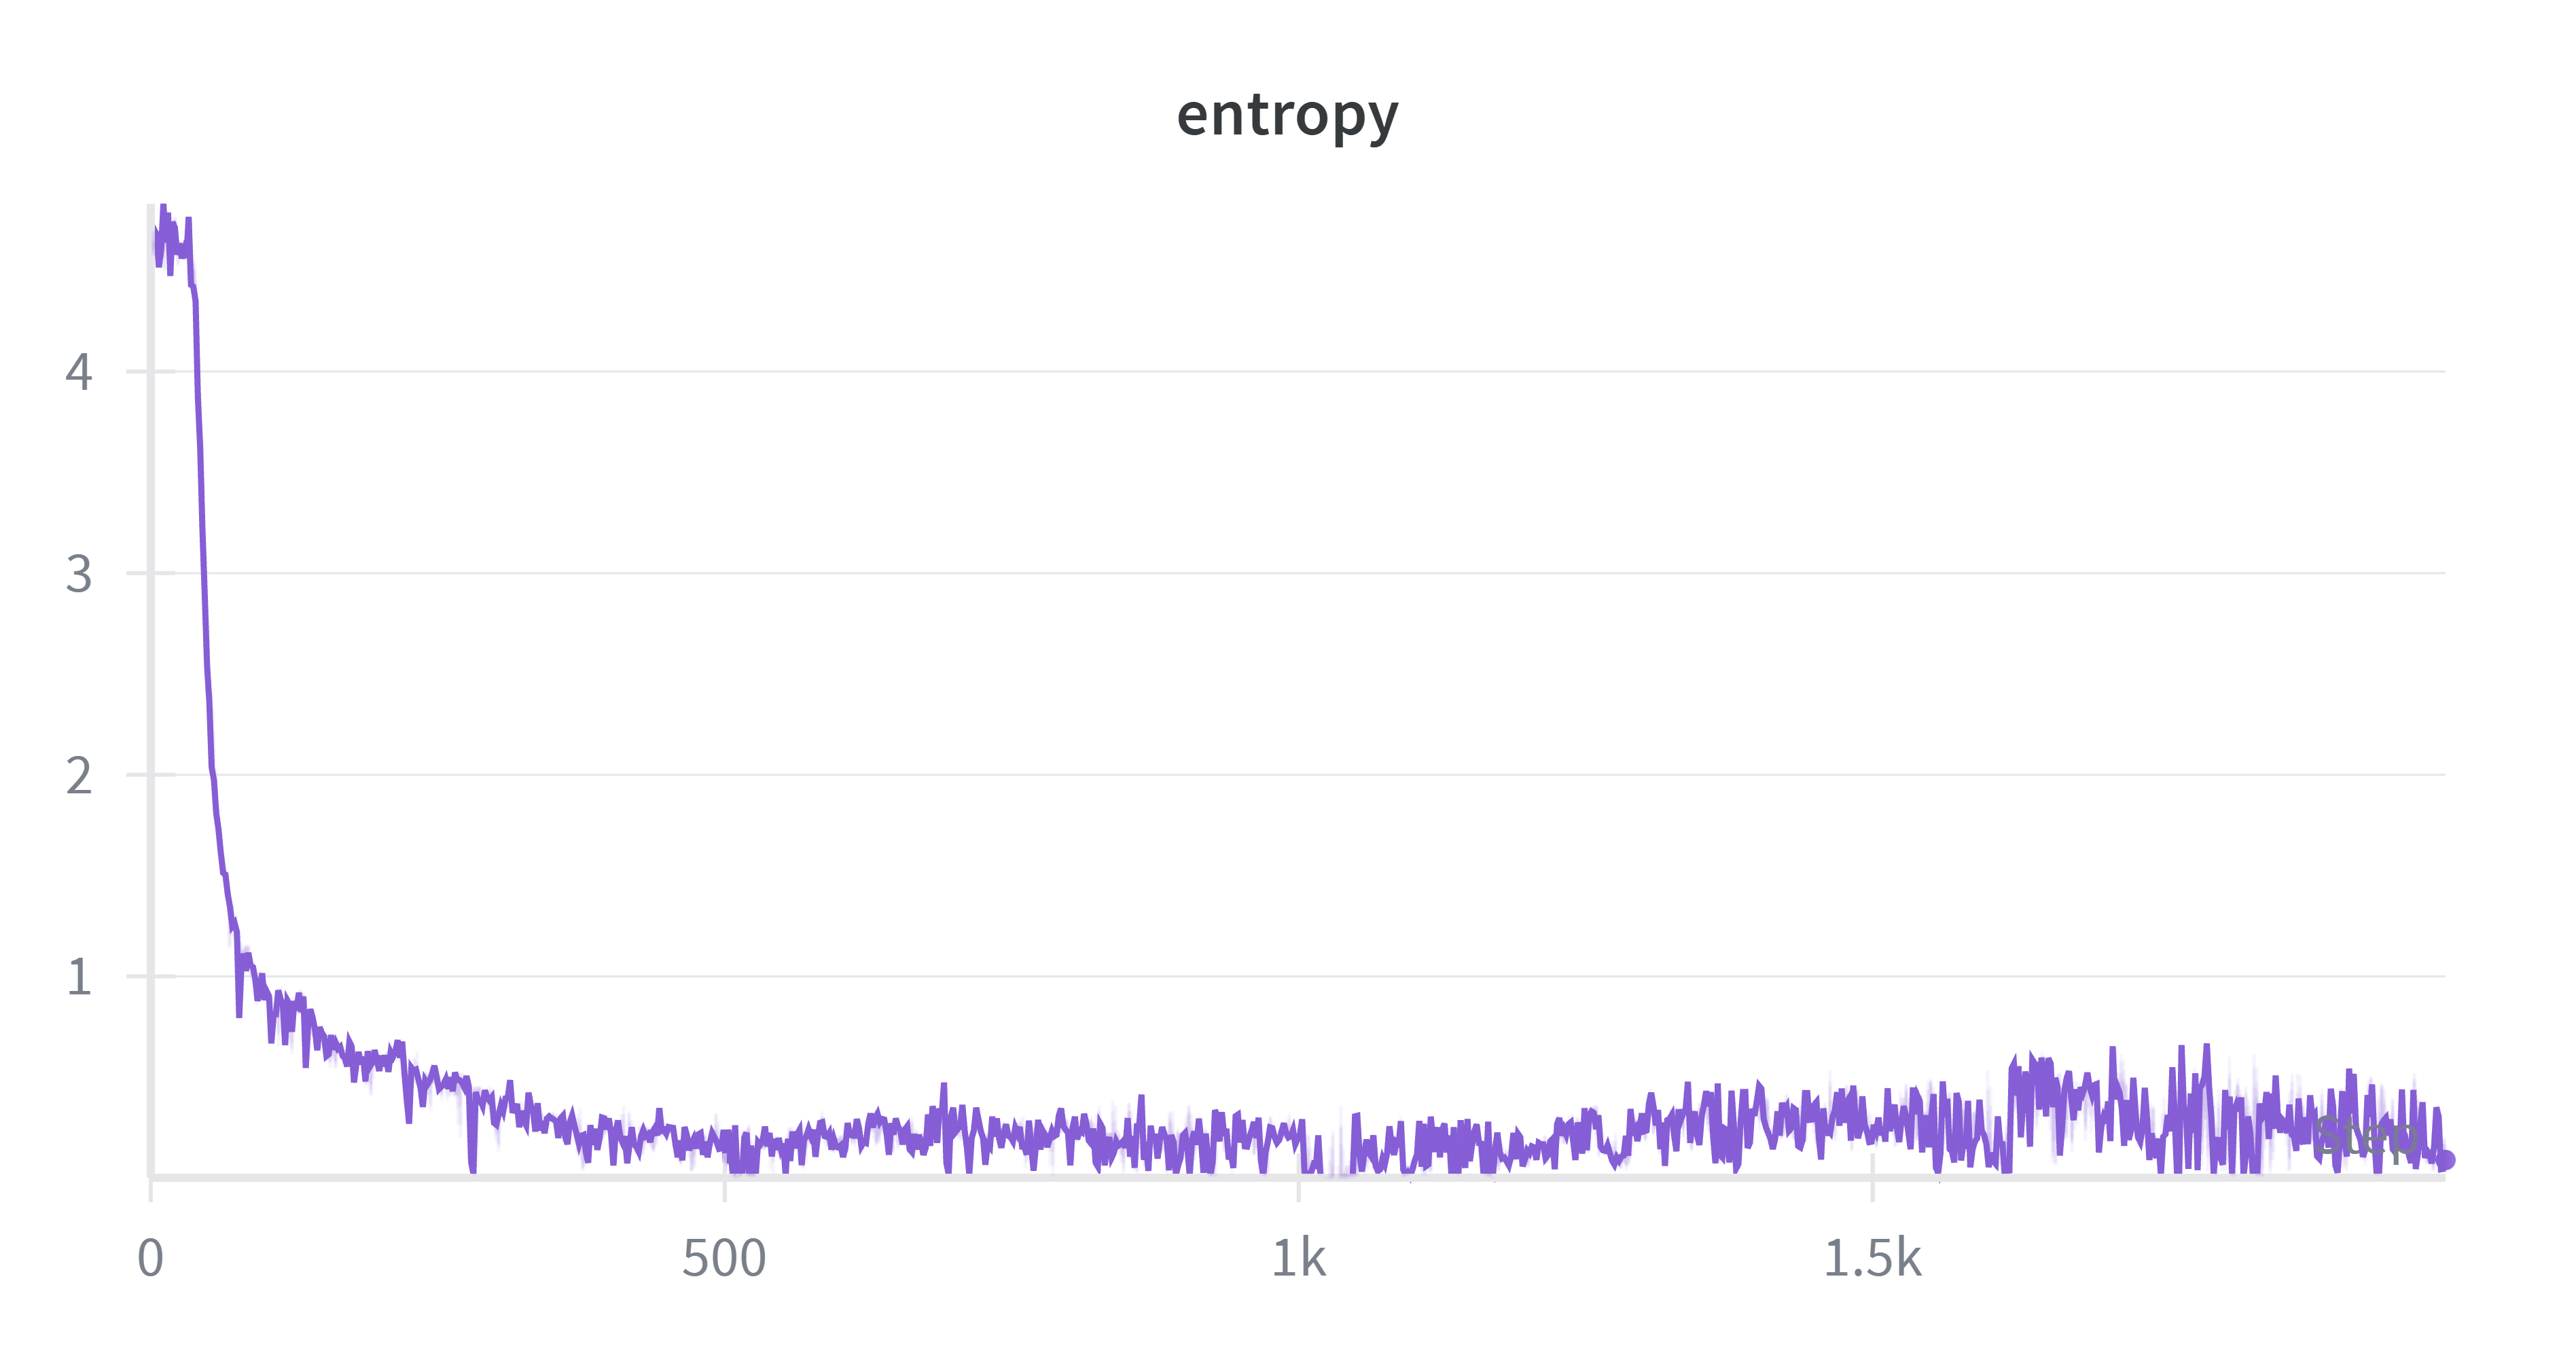
\includegraphics[width=\linewidth]{baseline_cnn_entropy.png}
        \caption{Baseline CNN}
    \end{subfigure}
    \hfill
    \begin{subfigure}{0.32\textwidth}
        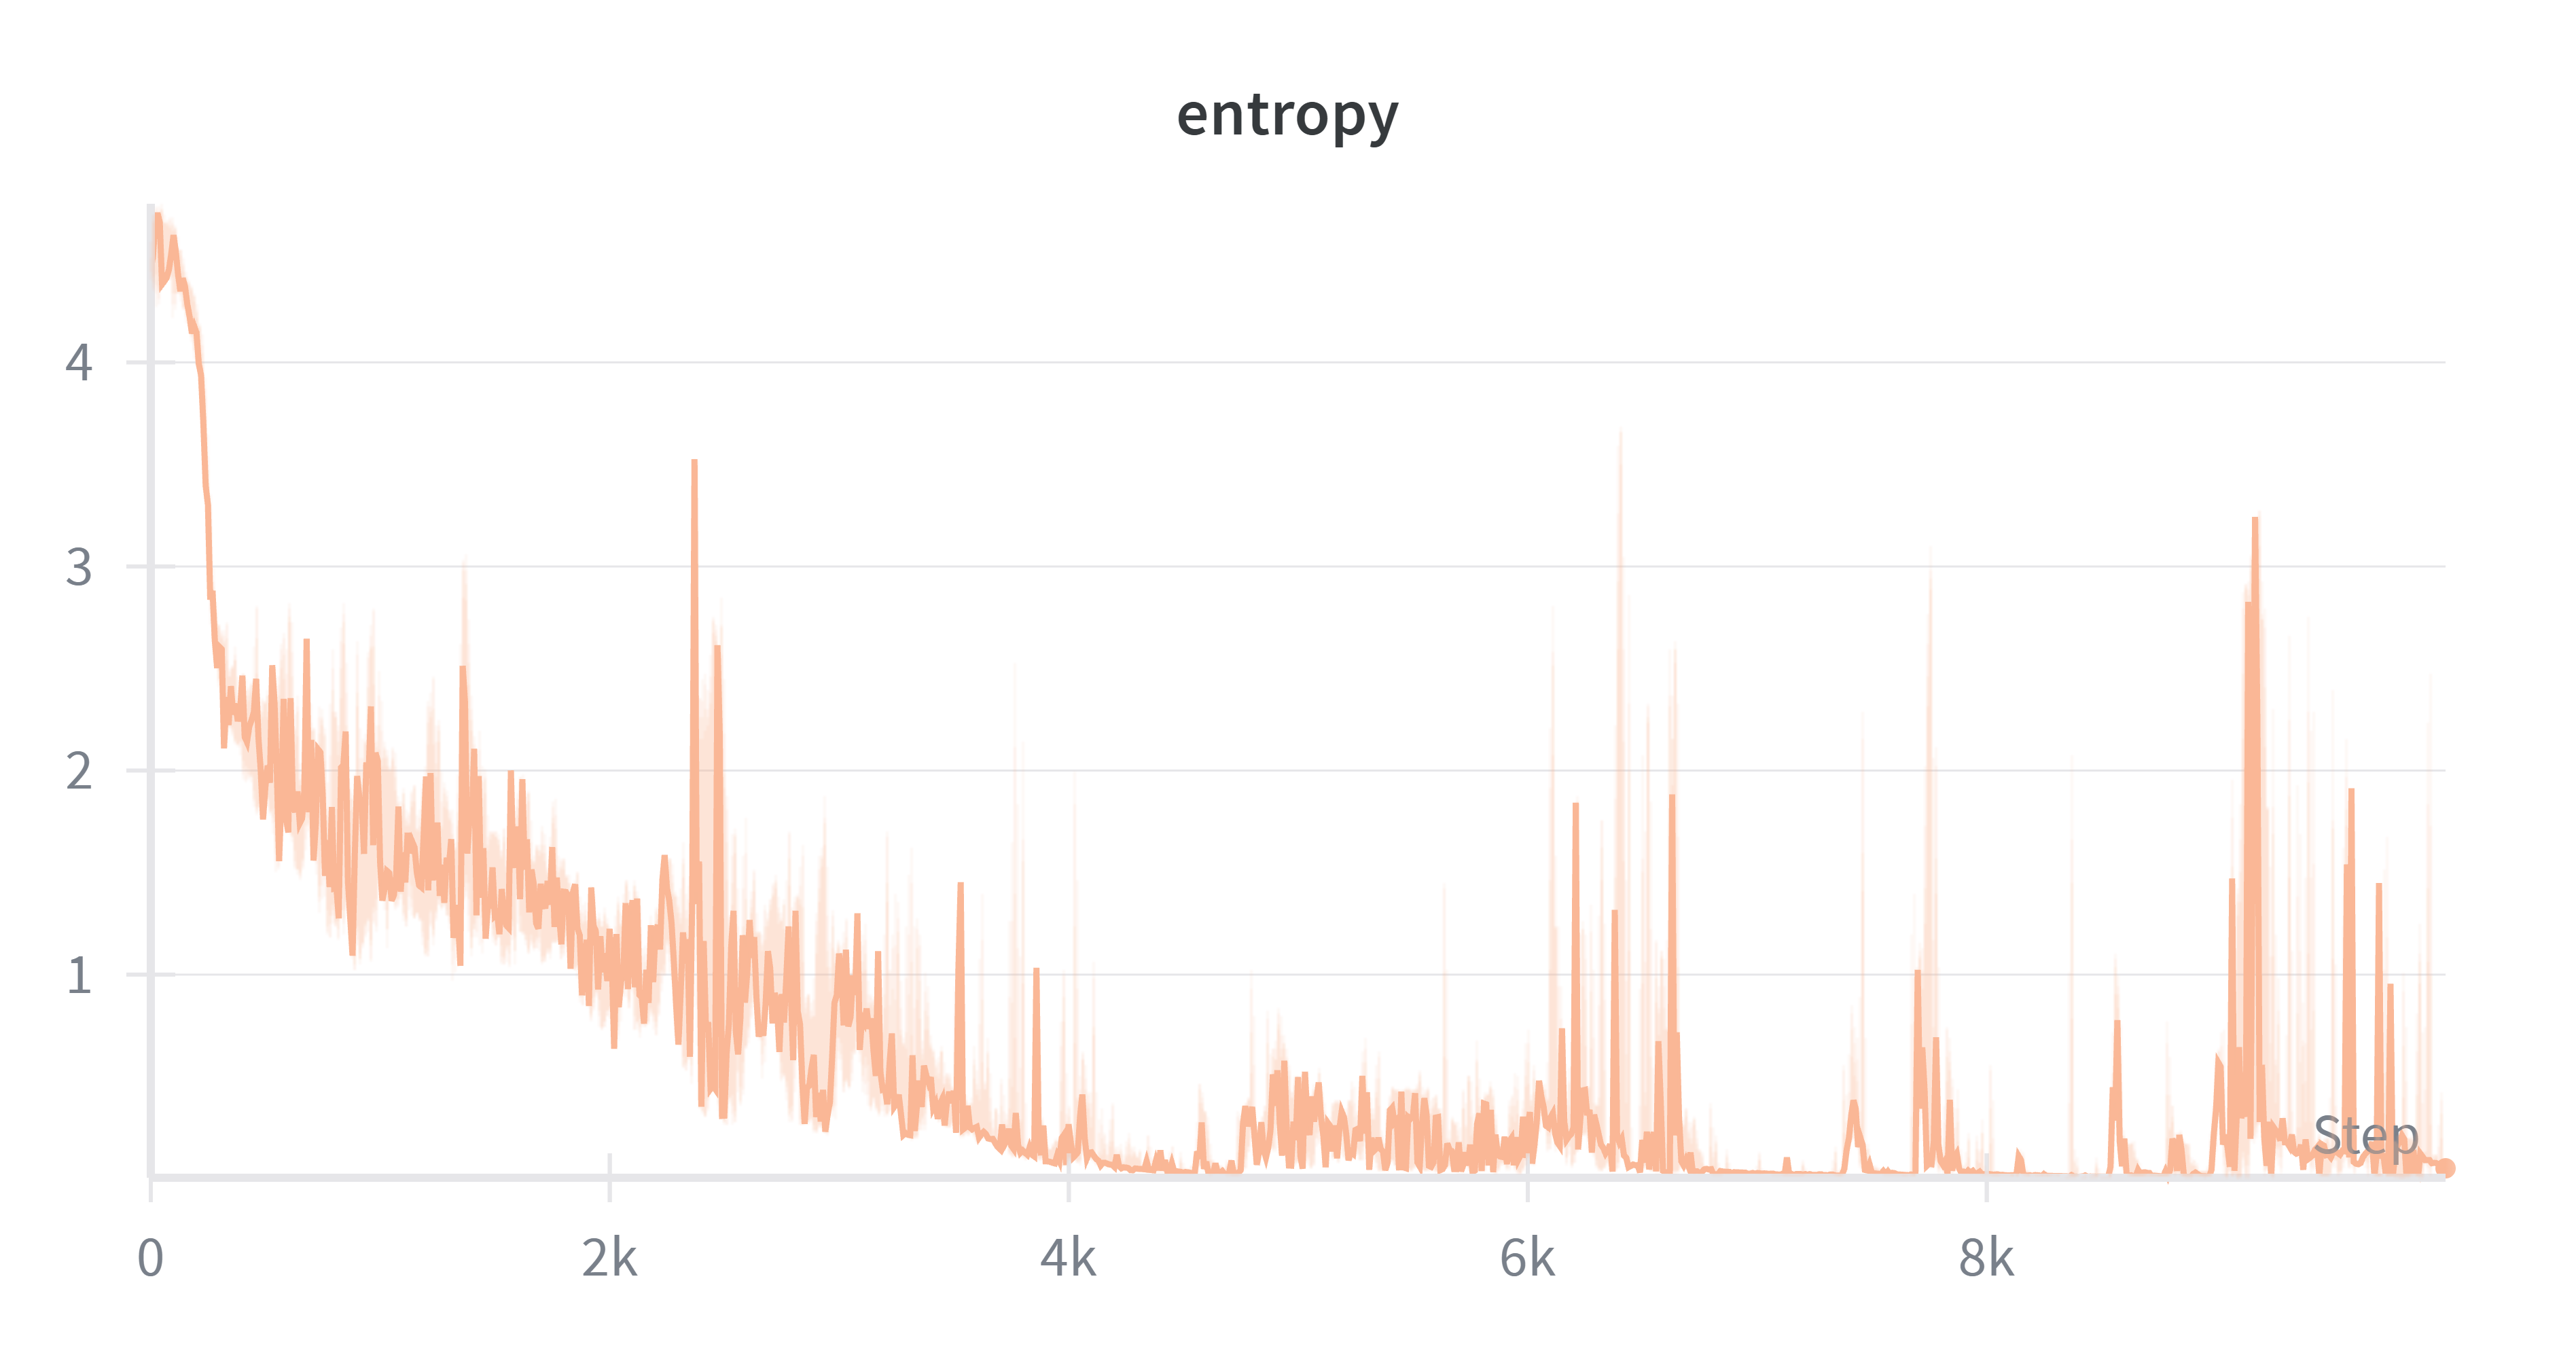
\includegraphics[width=\linewidth]{attention_entropy.png}
        \caption{Attention Actor}
    \end{subfigure}
    \hfill
    \begin{subfigure}{0.32\textwidth}
        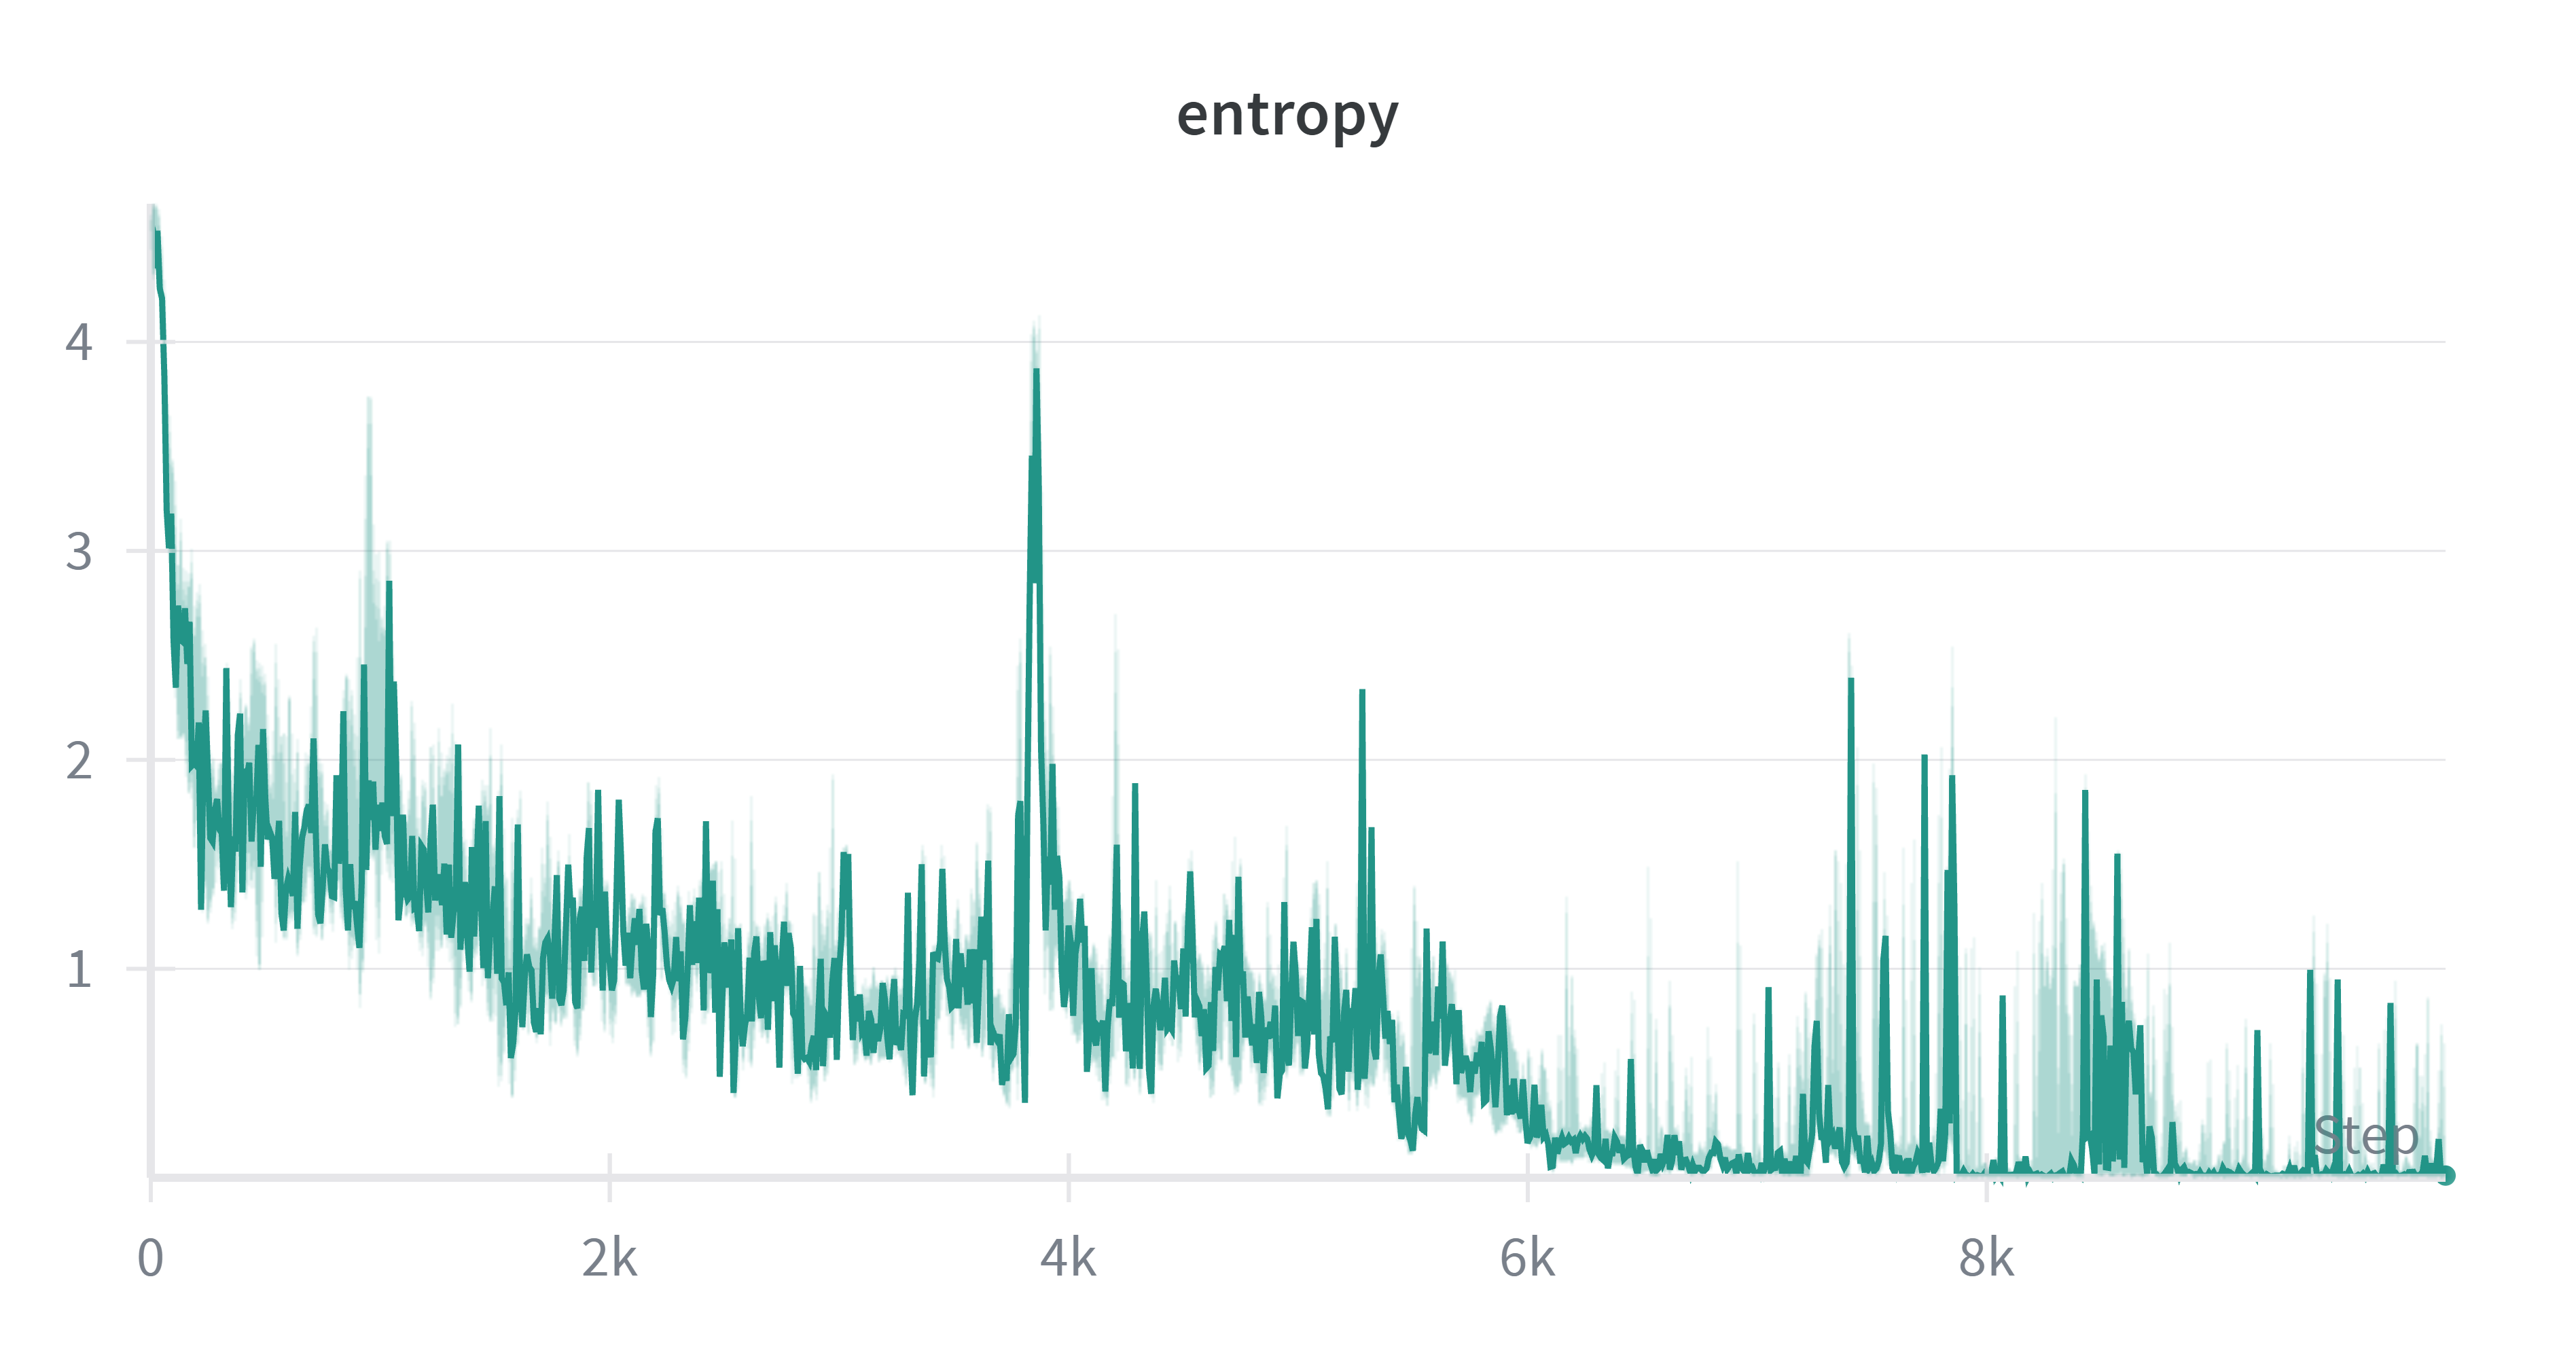
\includegraphics[width=\linewidth]{transformer_entropy.png}
        \caption{Transformer Actor}
    \end{subfigure}
    \caption{三种架构的策略熵变化趋势对比}
    \label{fig:entropy_comparison}
\end{figure}

\textbf{分析：}
\begin{itemize}
    \item \textbf{Baseline CNN}（左图）：熵值在训练初期（约前 1000 episodes）迅速坍塌至 0 附近。这表明模型极快地陷入了确定性策略，虽然收敛速度快，但也意味着它可能过早地放弃了对更优策略的探索（Premature Convergence）。
    \item \textbf{Attention Actor}（中图）：熵值表现出极大的震荡性，且经常出现异常尖峰。这说明单纯在 CNN 后附加 Attention 层可能引入了训练的不稳定性，导致策略分布难以稳定收敛。
    \item \textbf{Transformer Actor}（右图）：熵值呈现出缓慢且平稳的下降趋势，在整个 10000 轮训练中始终维持在 0 以上。这意味着 Transformer 始终保持着一定的探索能力，这种“持续探索”的特性是其最终在胜率上超越 CNN 的关键原因。
\end{itemize}

\subsubsection{价值网络损失 (Critic Loss) 对比}
Critic Loss ($L = MSE(R + \gamma Q_{next}, Q_{cur})$) 反映了价值网络对自己预测准确性的评估。

\begin{figure}[H]
    \centering
    \begin{subfigure}{0.32\textwidth}
        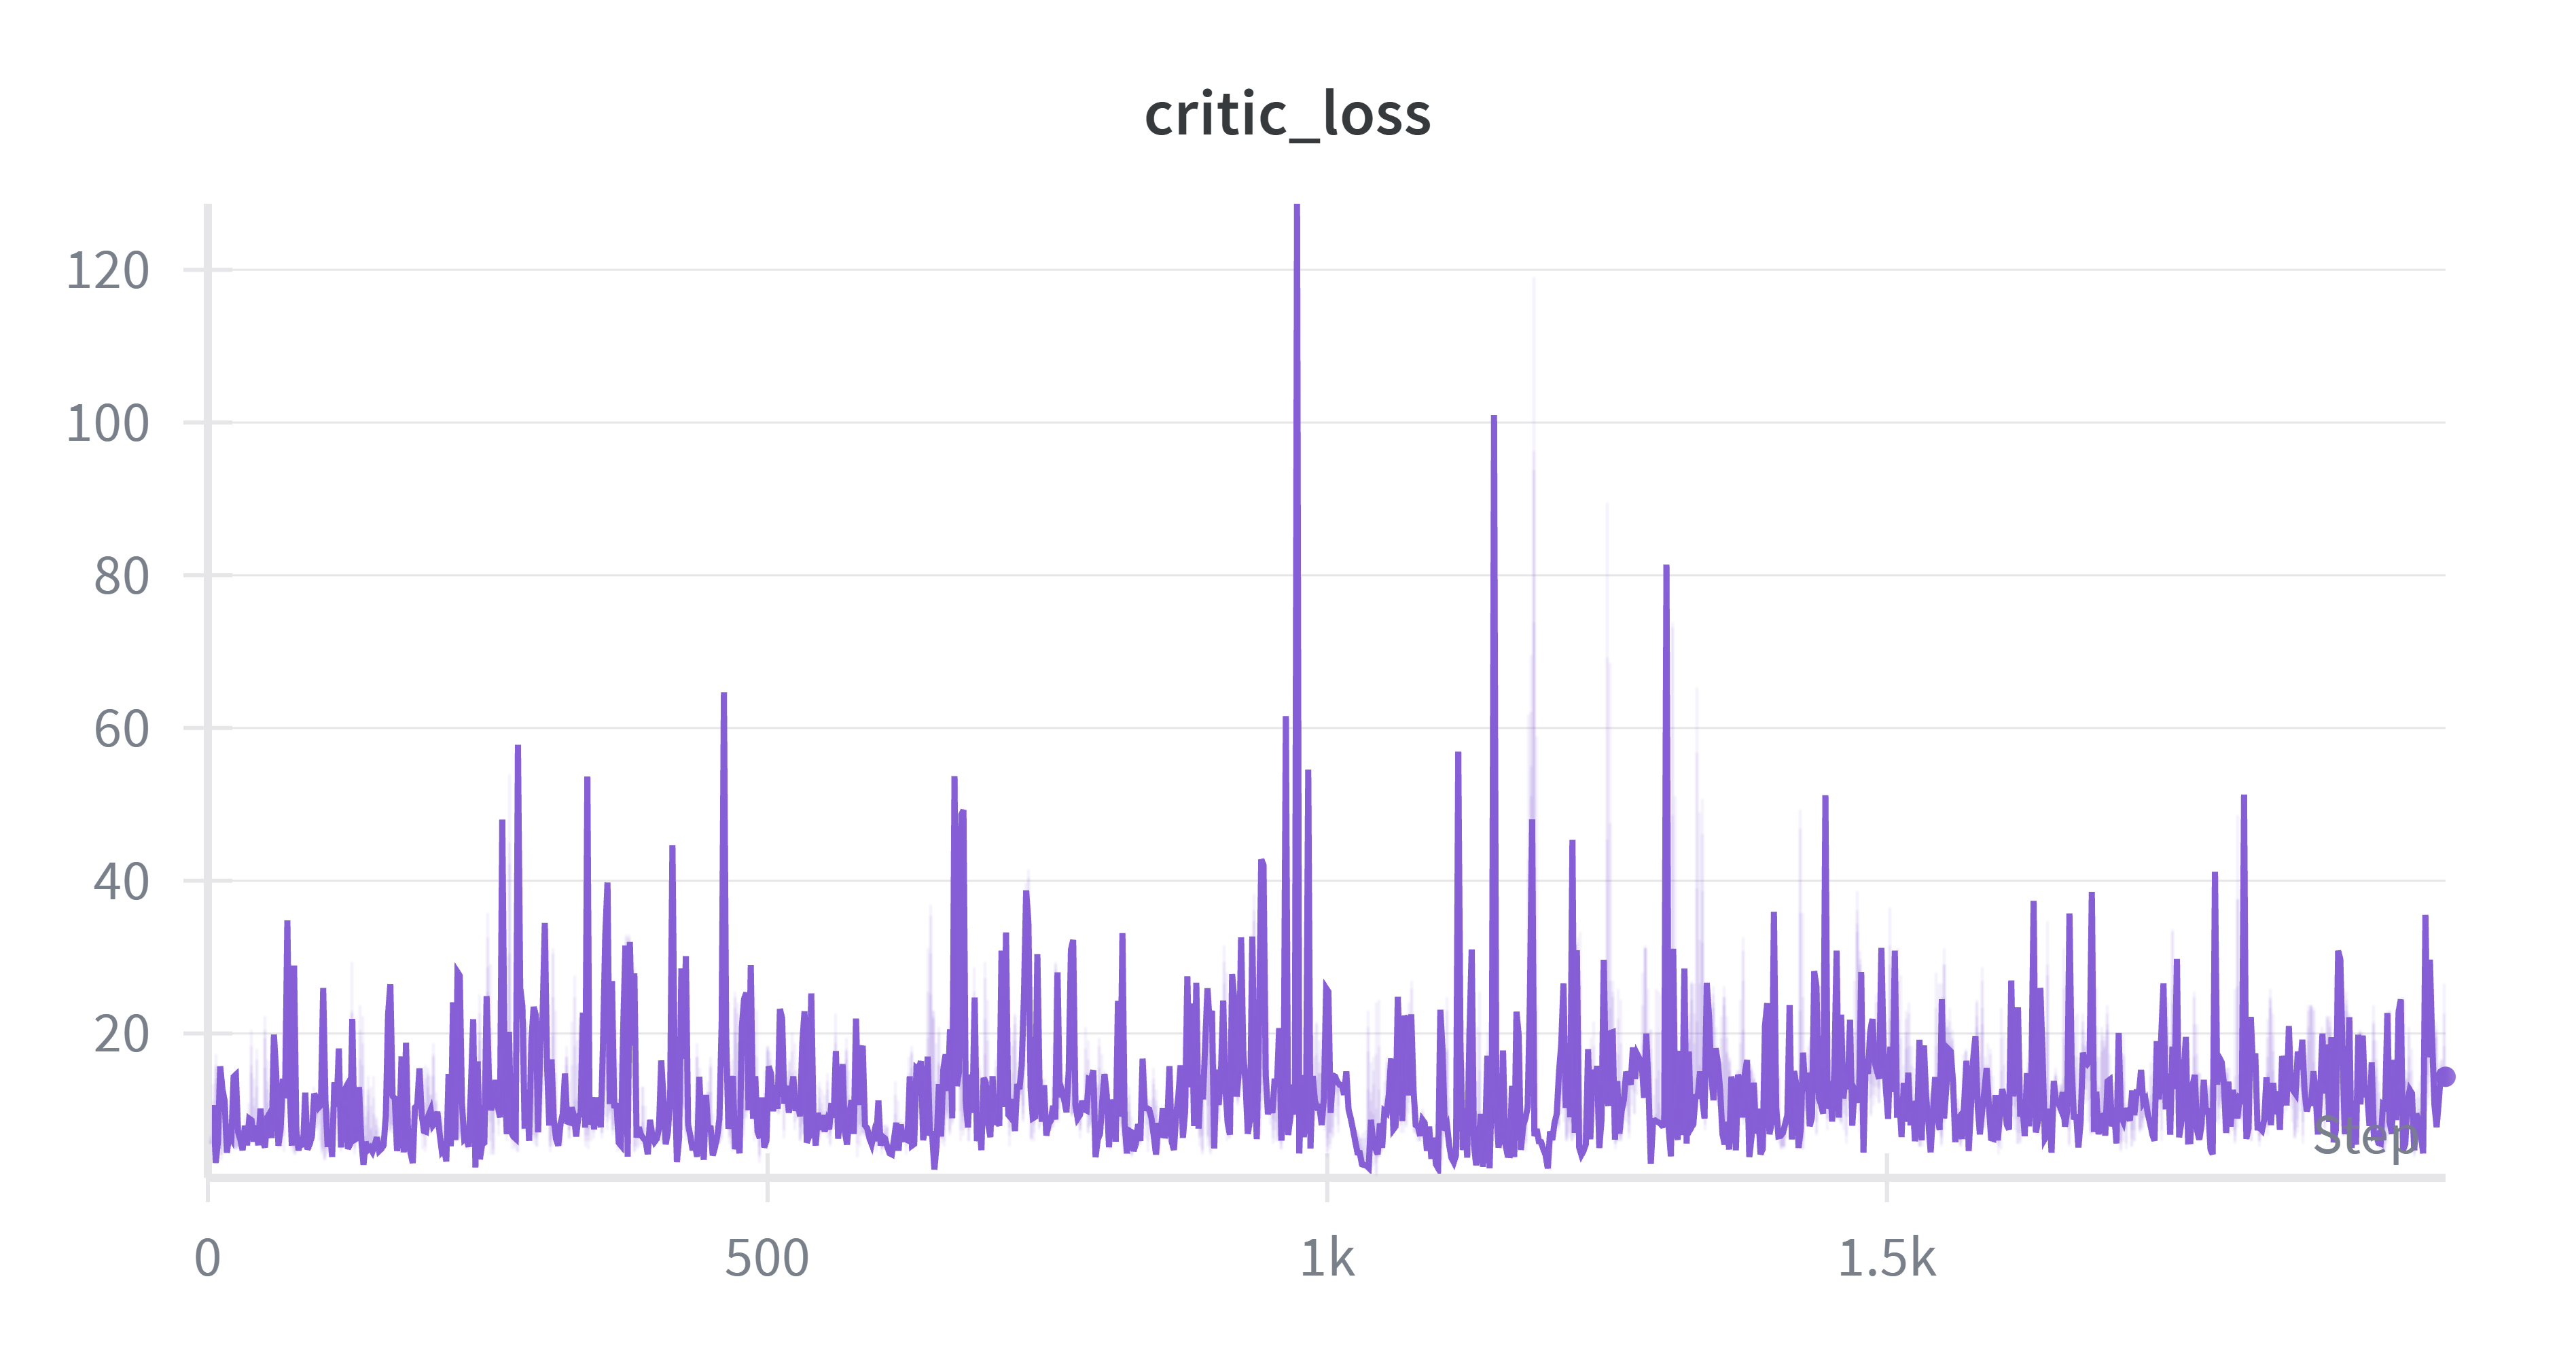
\includegraphics[width=\linewidth]{baseline_cnn_critic_loss.png}
        \caption{Baseline CNN}
    \end{subfigure}
    \hfill
    \begin{subfigure}{0.32\textwidth}
        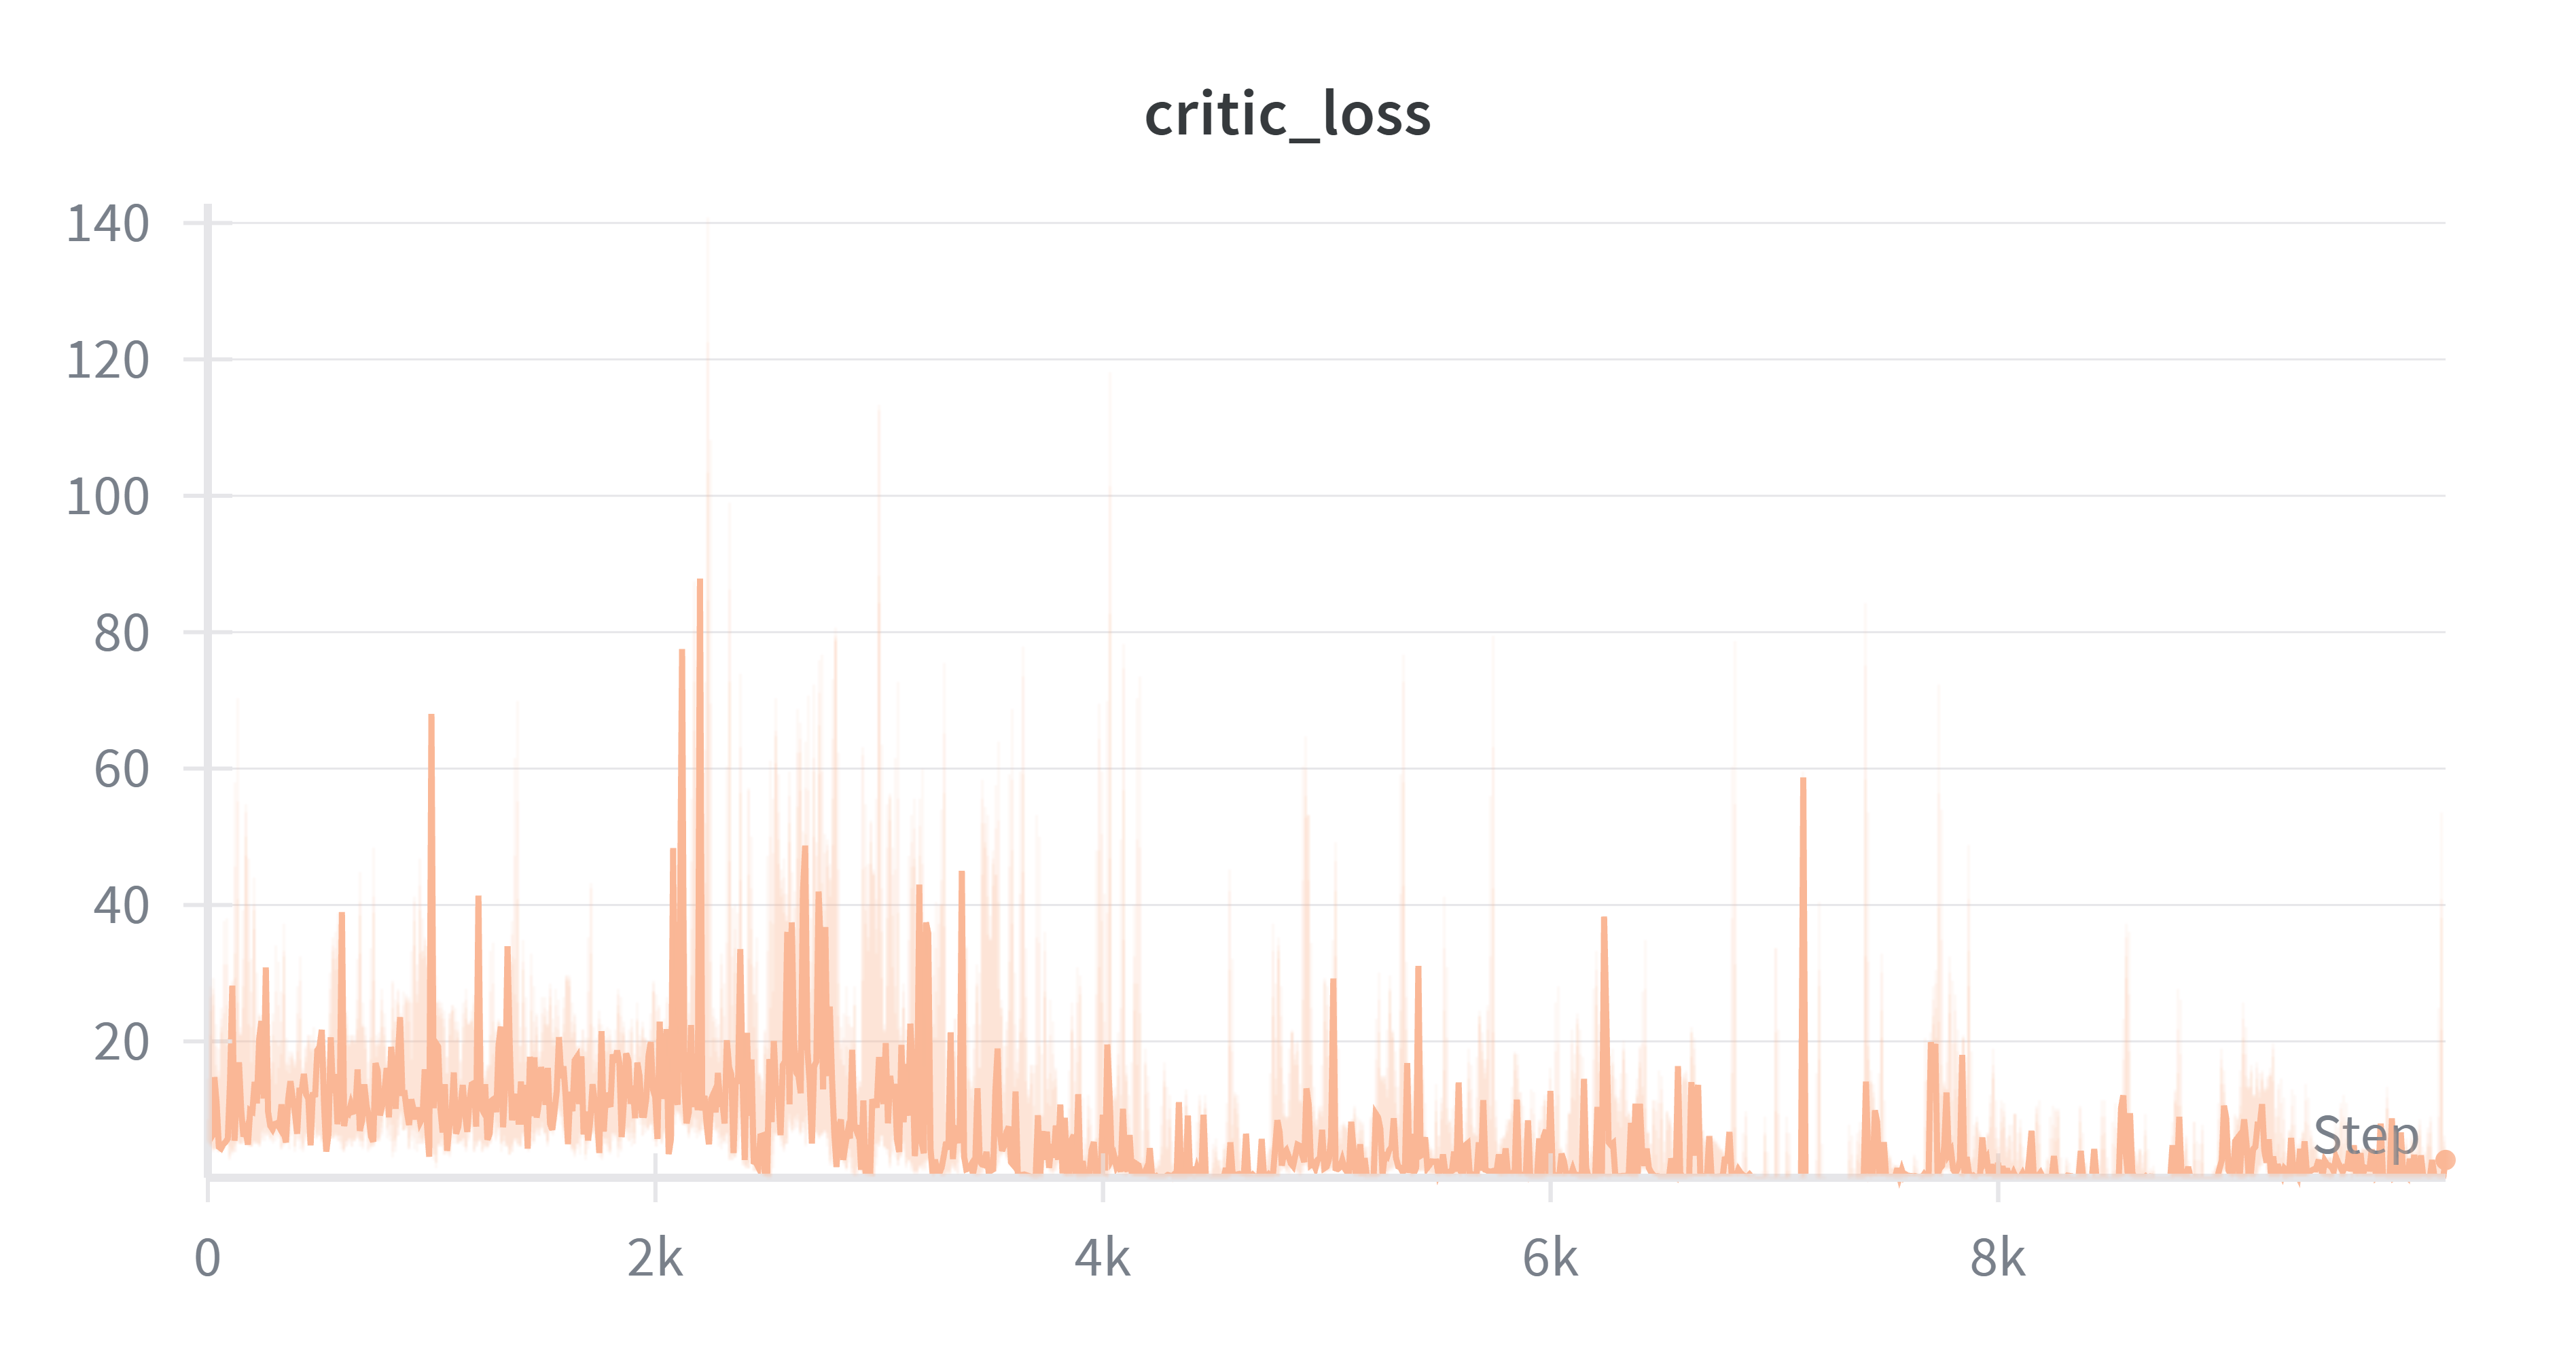
\includegraphics[width=\linewidth]{attention_critic_loss.png}
        \caption{Attention Actor}
    \end{subfigure}
    \hfill
    \begin{subfigure}{0.32\textwidth}
        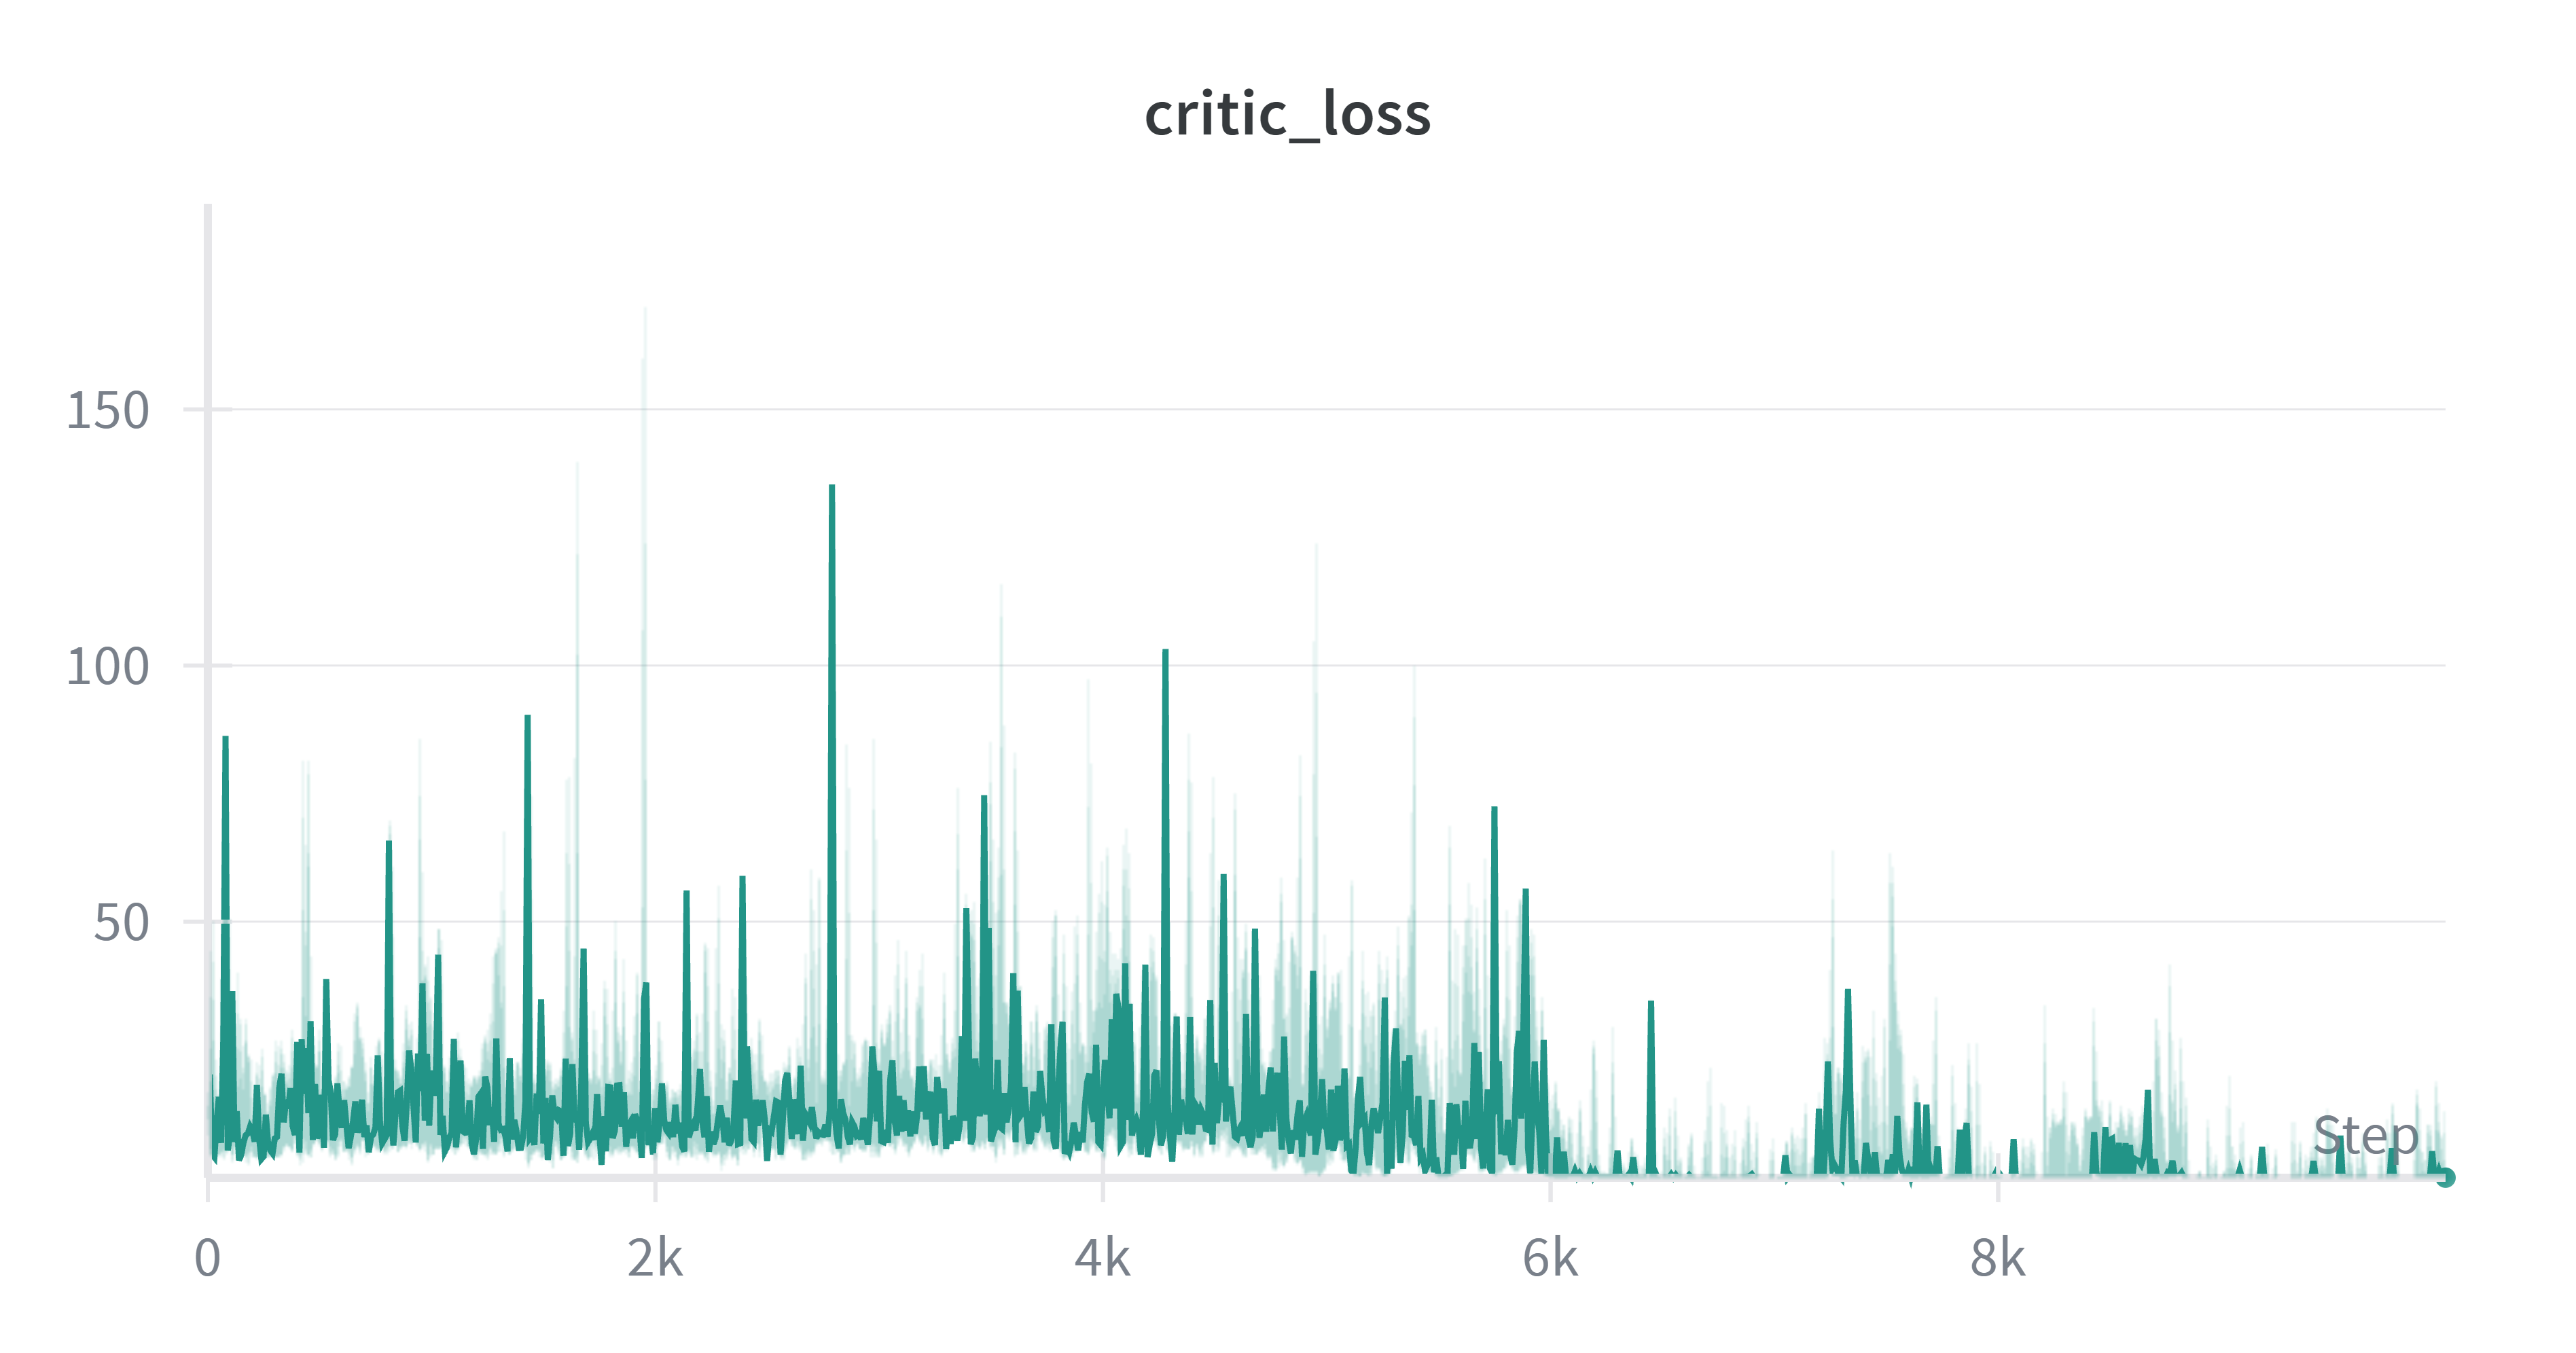
\includegraphics[width=\linewidth]{transformer_critic_loss.png}
        \caption{Transformer Actor}
    \end{subfigure}
    \caption{三种架构的 Critic Loss 变化趋势对比}
    \label{fig:critic_loss_comparison}
\end{figure}

\textbf{分析：}
\begin{itemize}
    \item \textbf{Baseline CNN}：Critic Loss 迅速降低并保持在极低水平。这与熵的快速坍塌一致——由于 Actor 总是走“老路”，Critic 面对的状态非常单一，因此很容易“猜对”价值，但这是一种虚假的“准确”。
    \item \textbf{Transformer Actor}：Critic Loss 在训练后期仍保持一定的波动。这是良性的信号：由于 Transformer Actor 持续探索新动作，Critic 不断被迫面对分布外（Out-of-Distribution）的新局面，从而推动价值网络不断修正和学习，最终获得更鲁棒的全局估值能力。
\end{itemize}

\subsubsection{策略网络损失 (Actor Loss) 对比}
Actor 的目标是最大化期望回报，代码中体现为最小化 $Loss = -\text{mean}(\log \pi(a|s) \cdot Q(s,a))$。

\begin{figure}[H]
    \centering
    \begin{subfigure}{0.32\textwidth}
        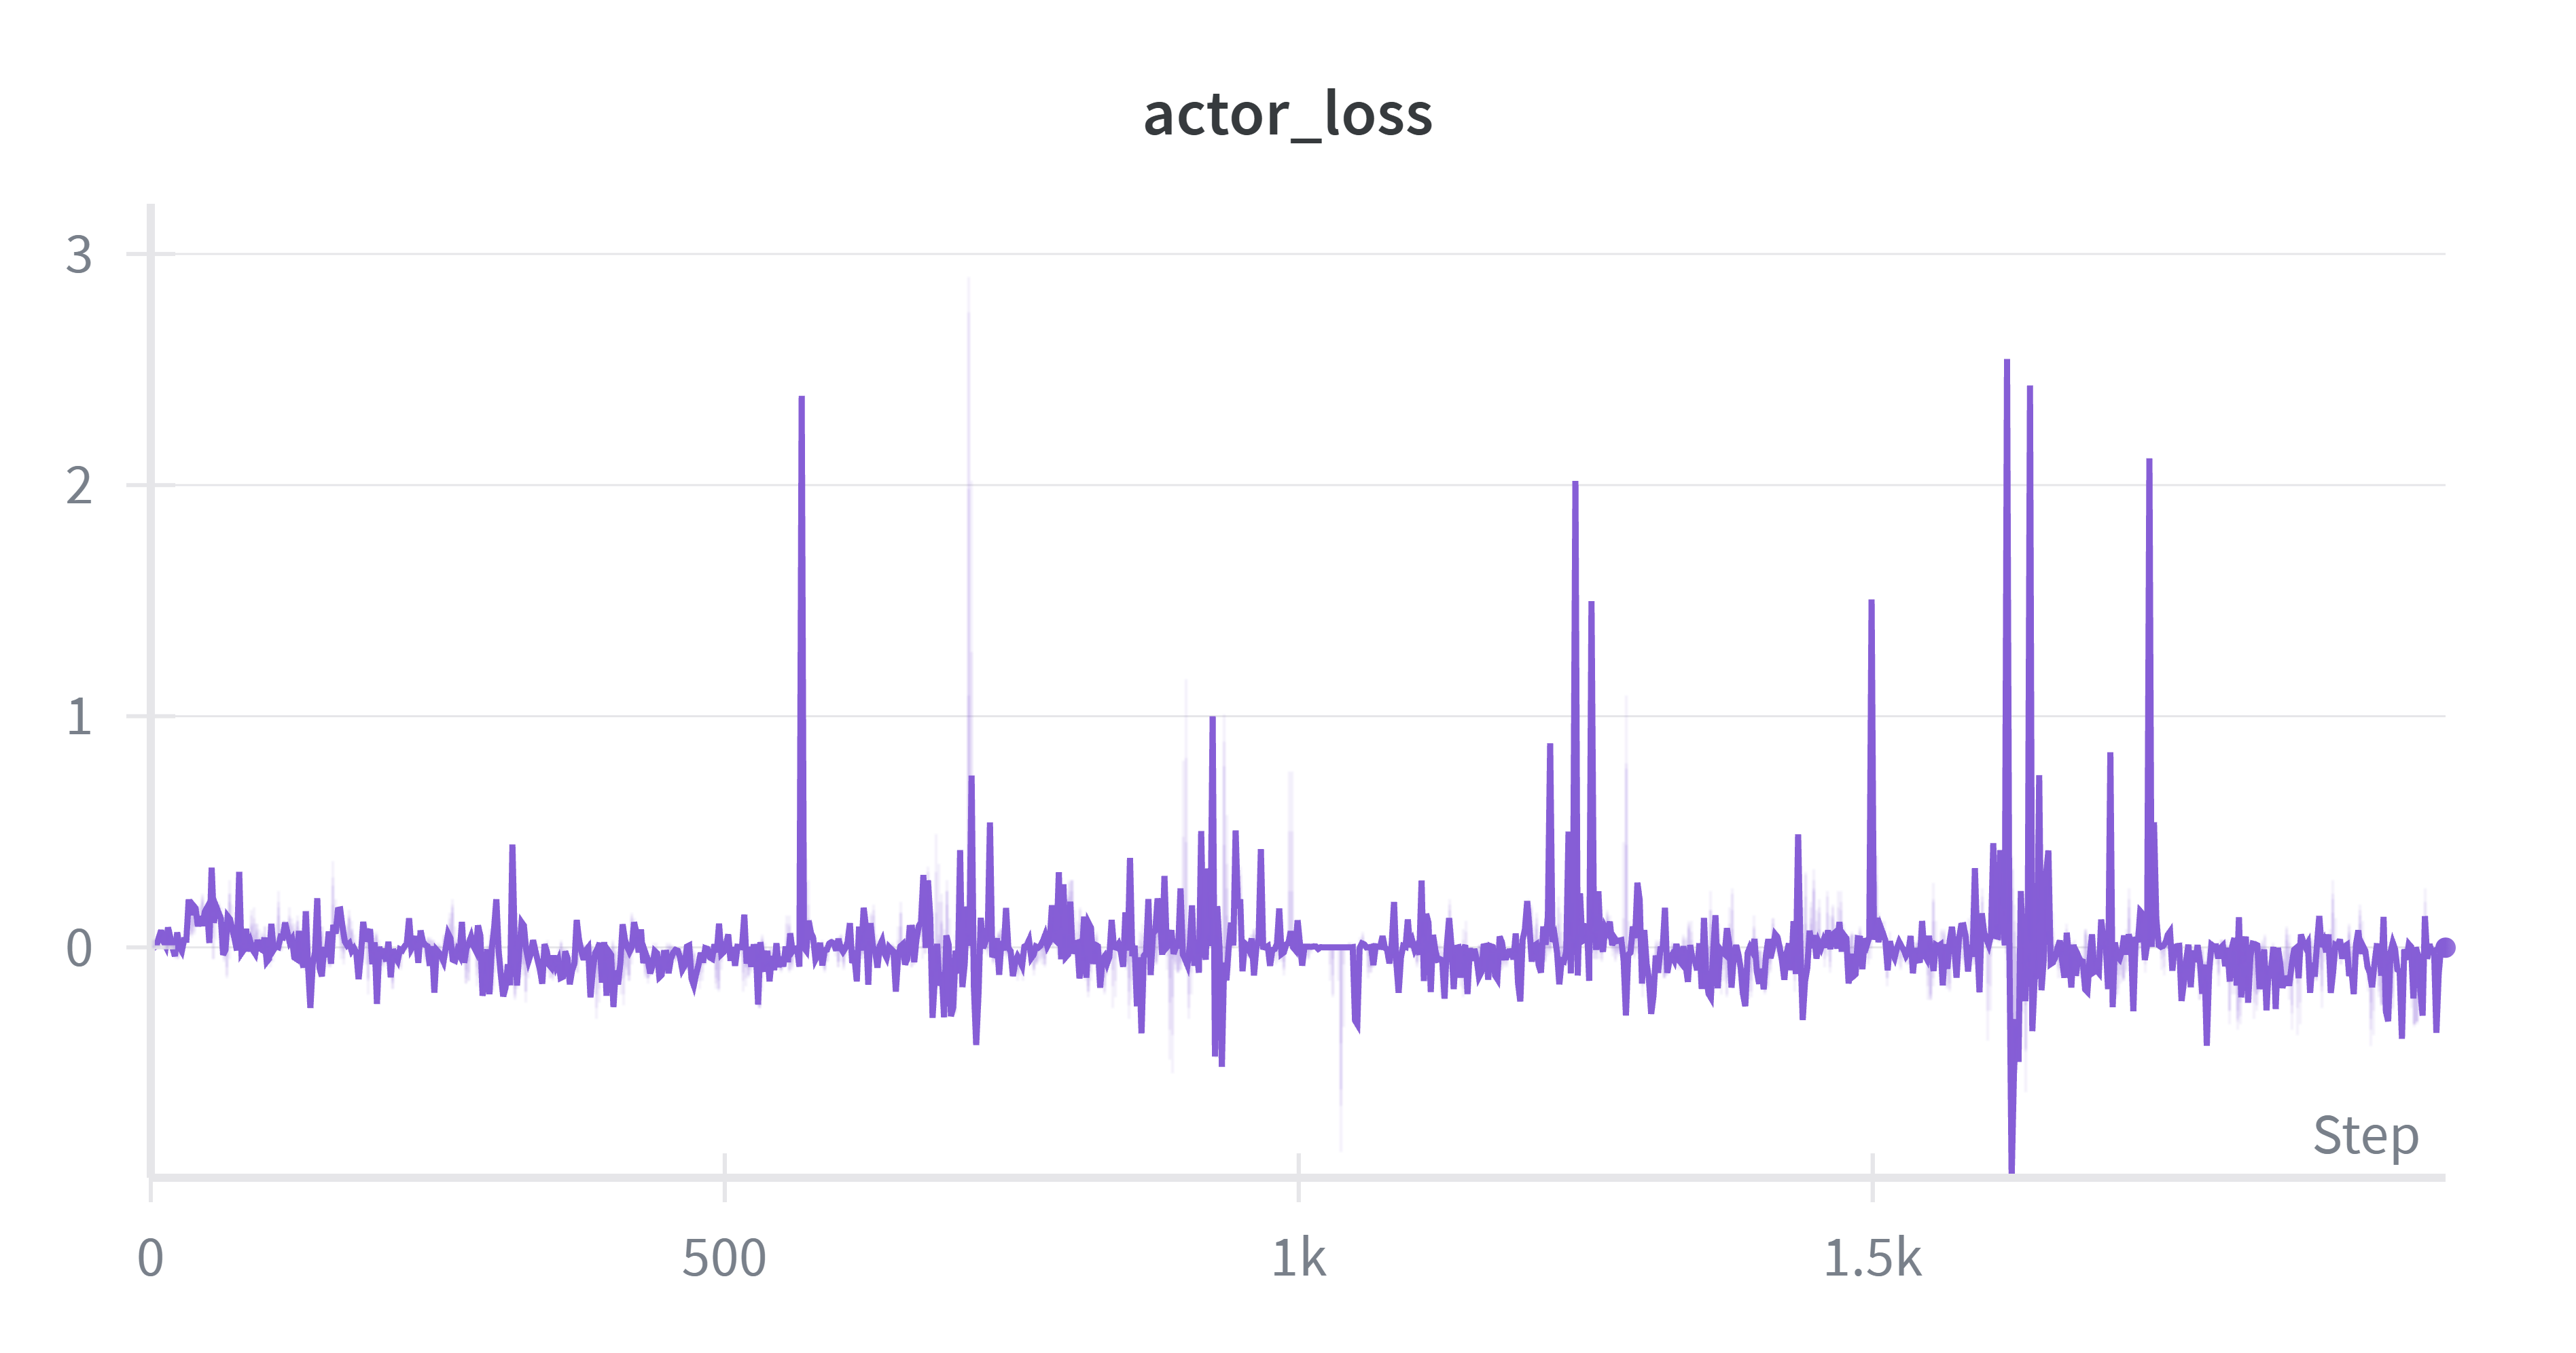
\includegraphics[width=\linewidth]{baseline_cnn_actor_loss.png}
        \caption{Baseline CNN}
    \end{subfigure}
    \hfill
    \begin{subfigure}{0.32\textwidth}
        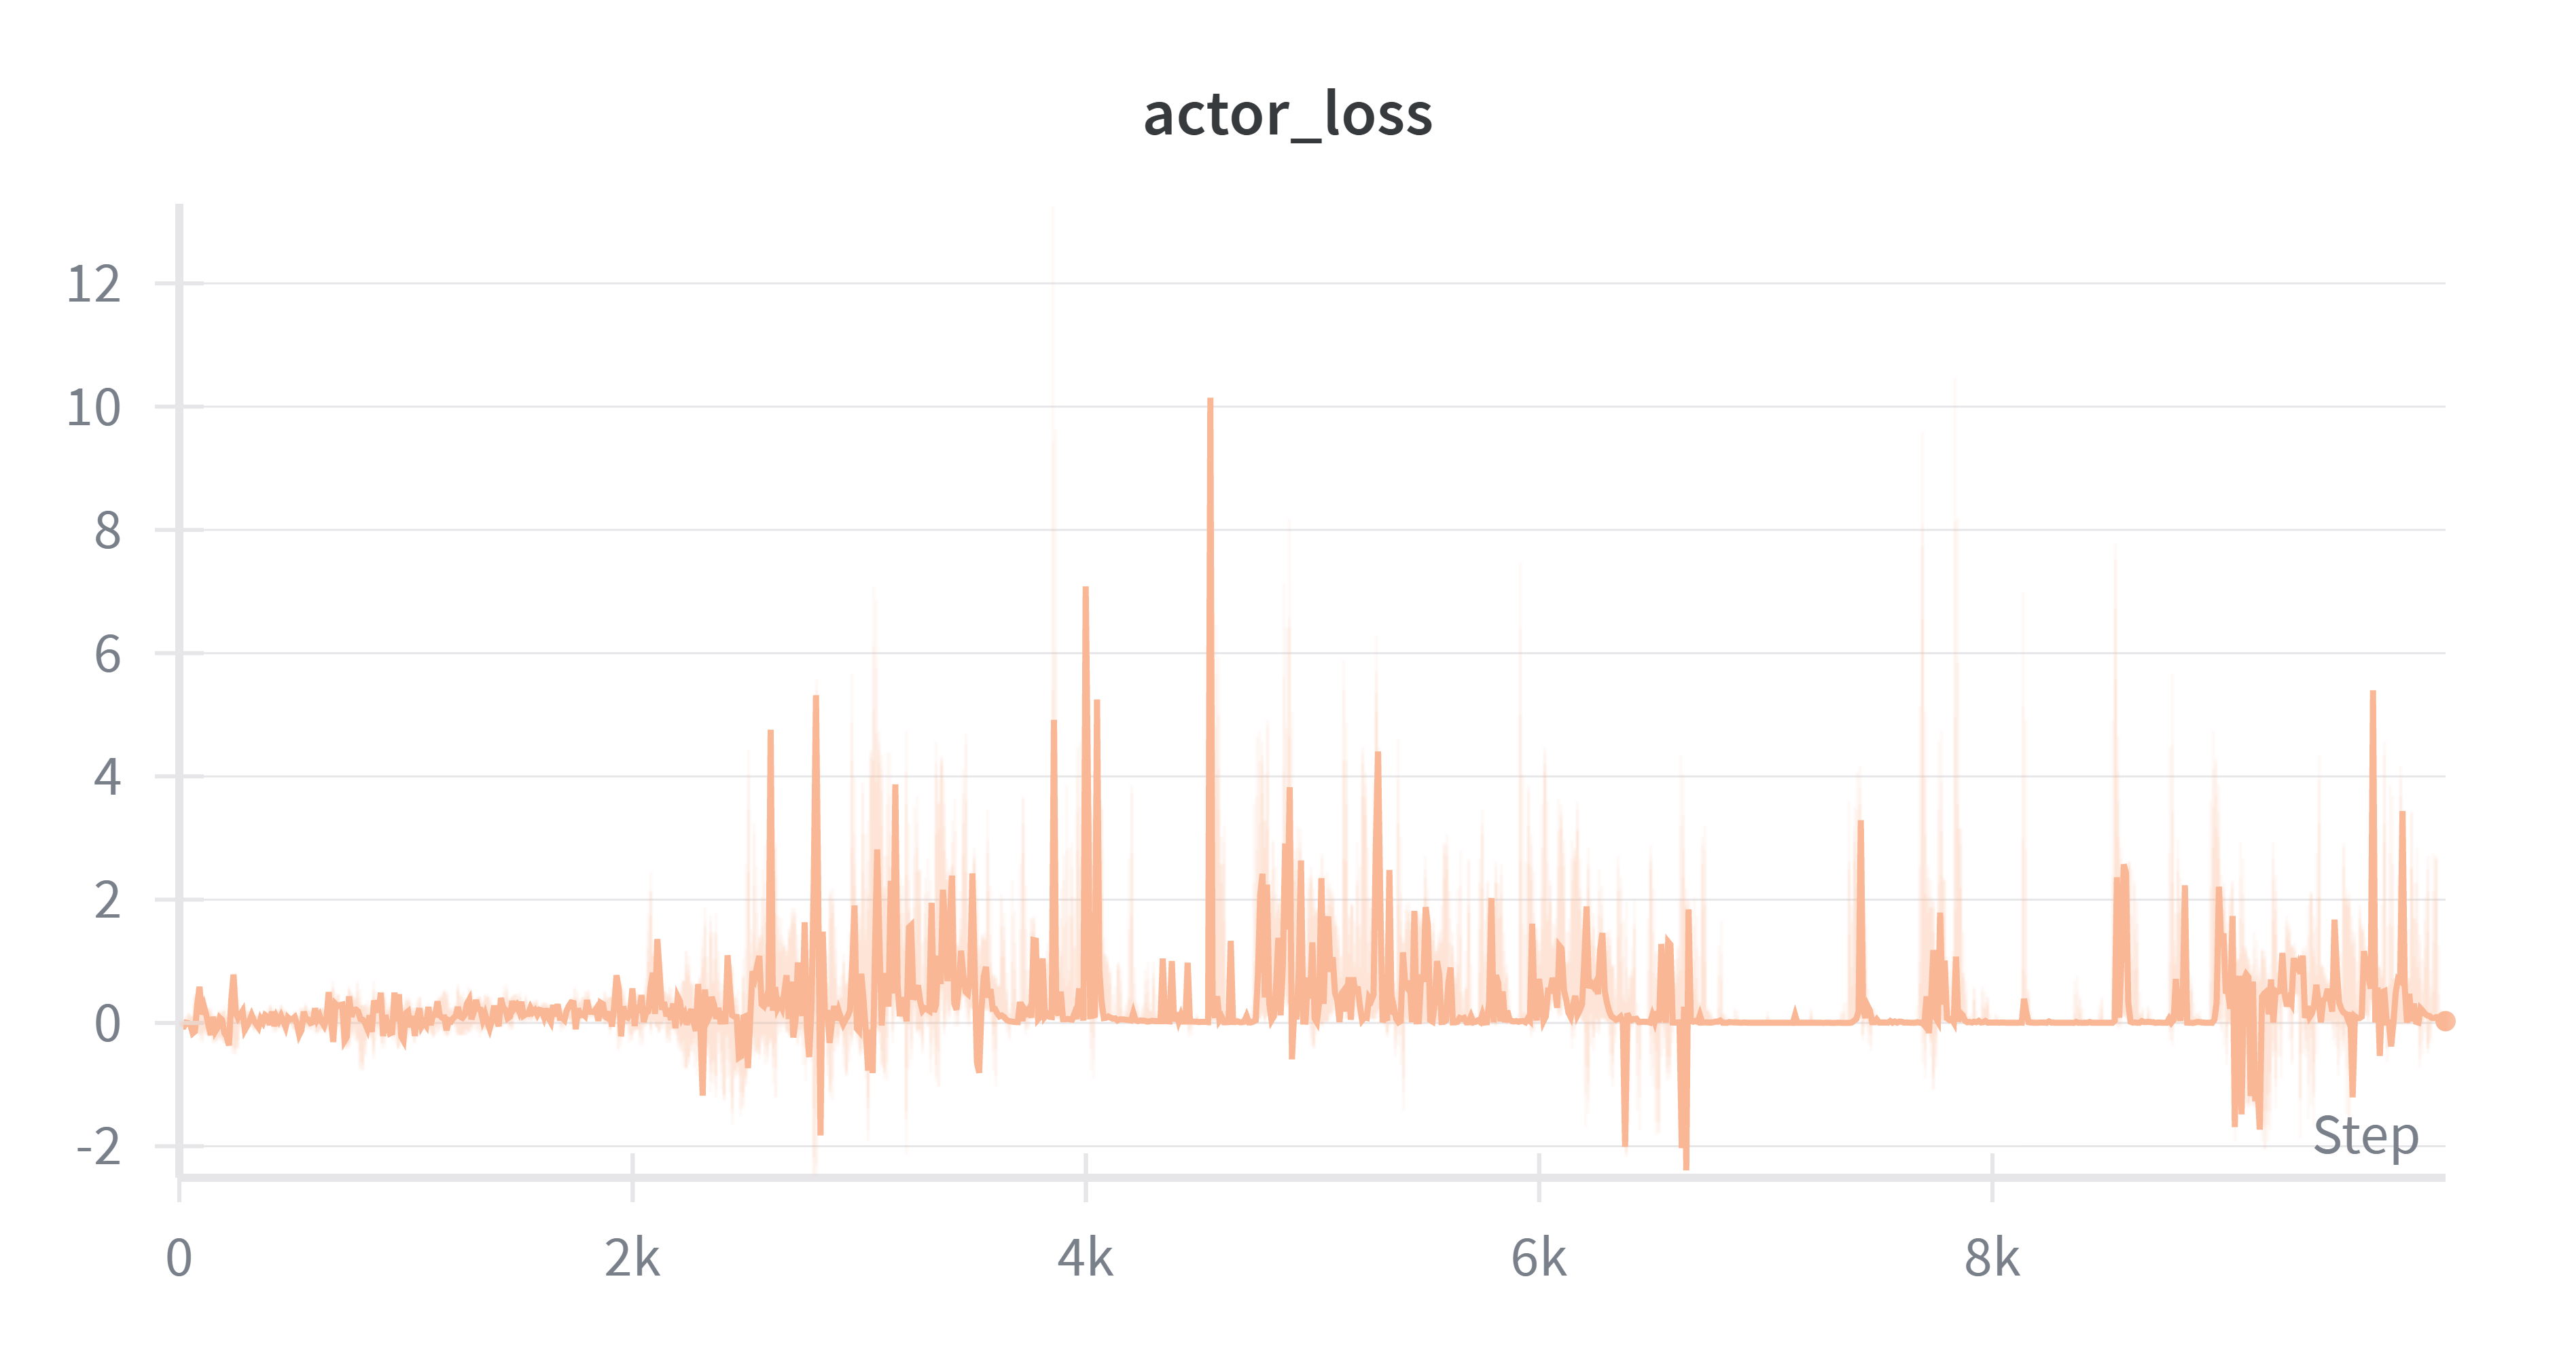
\includegraphics[width=\linewidth]{attention_actor_loss.png}
        \caption{Attention Actor}
    \end{subfigure}
    \hfill
    \begin{subfigure}{0.32\textwidth}
        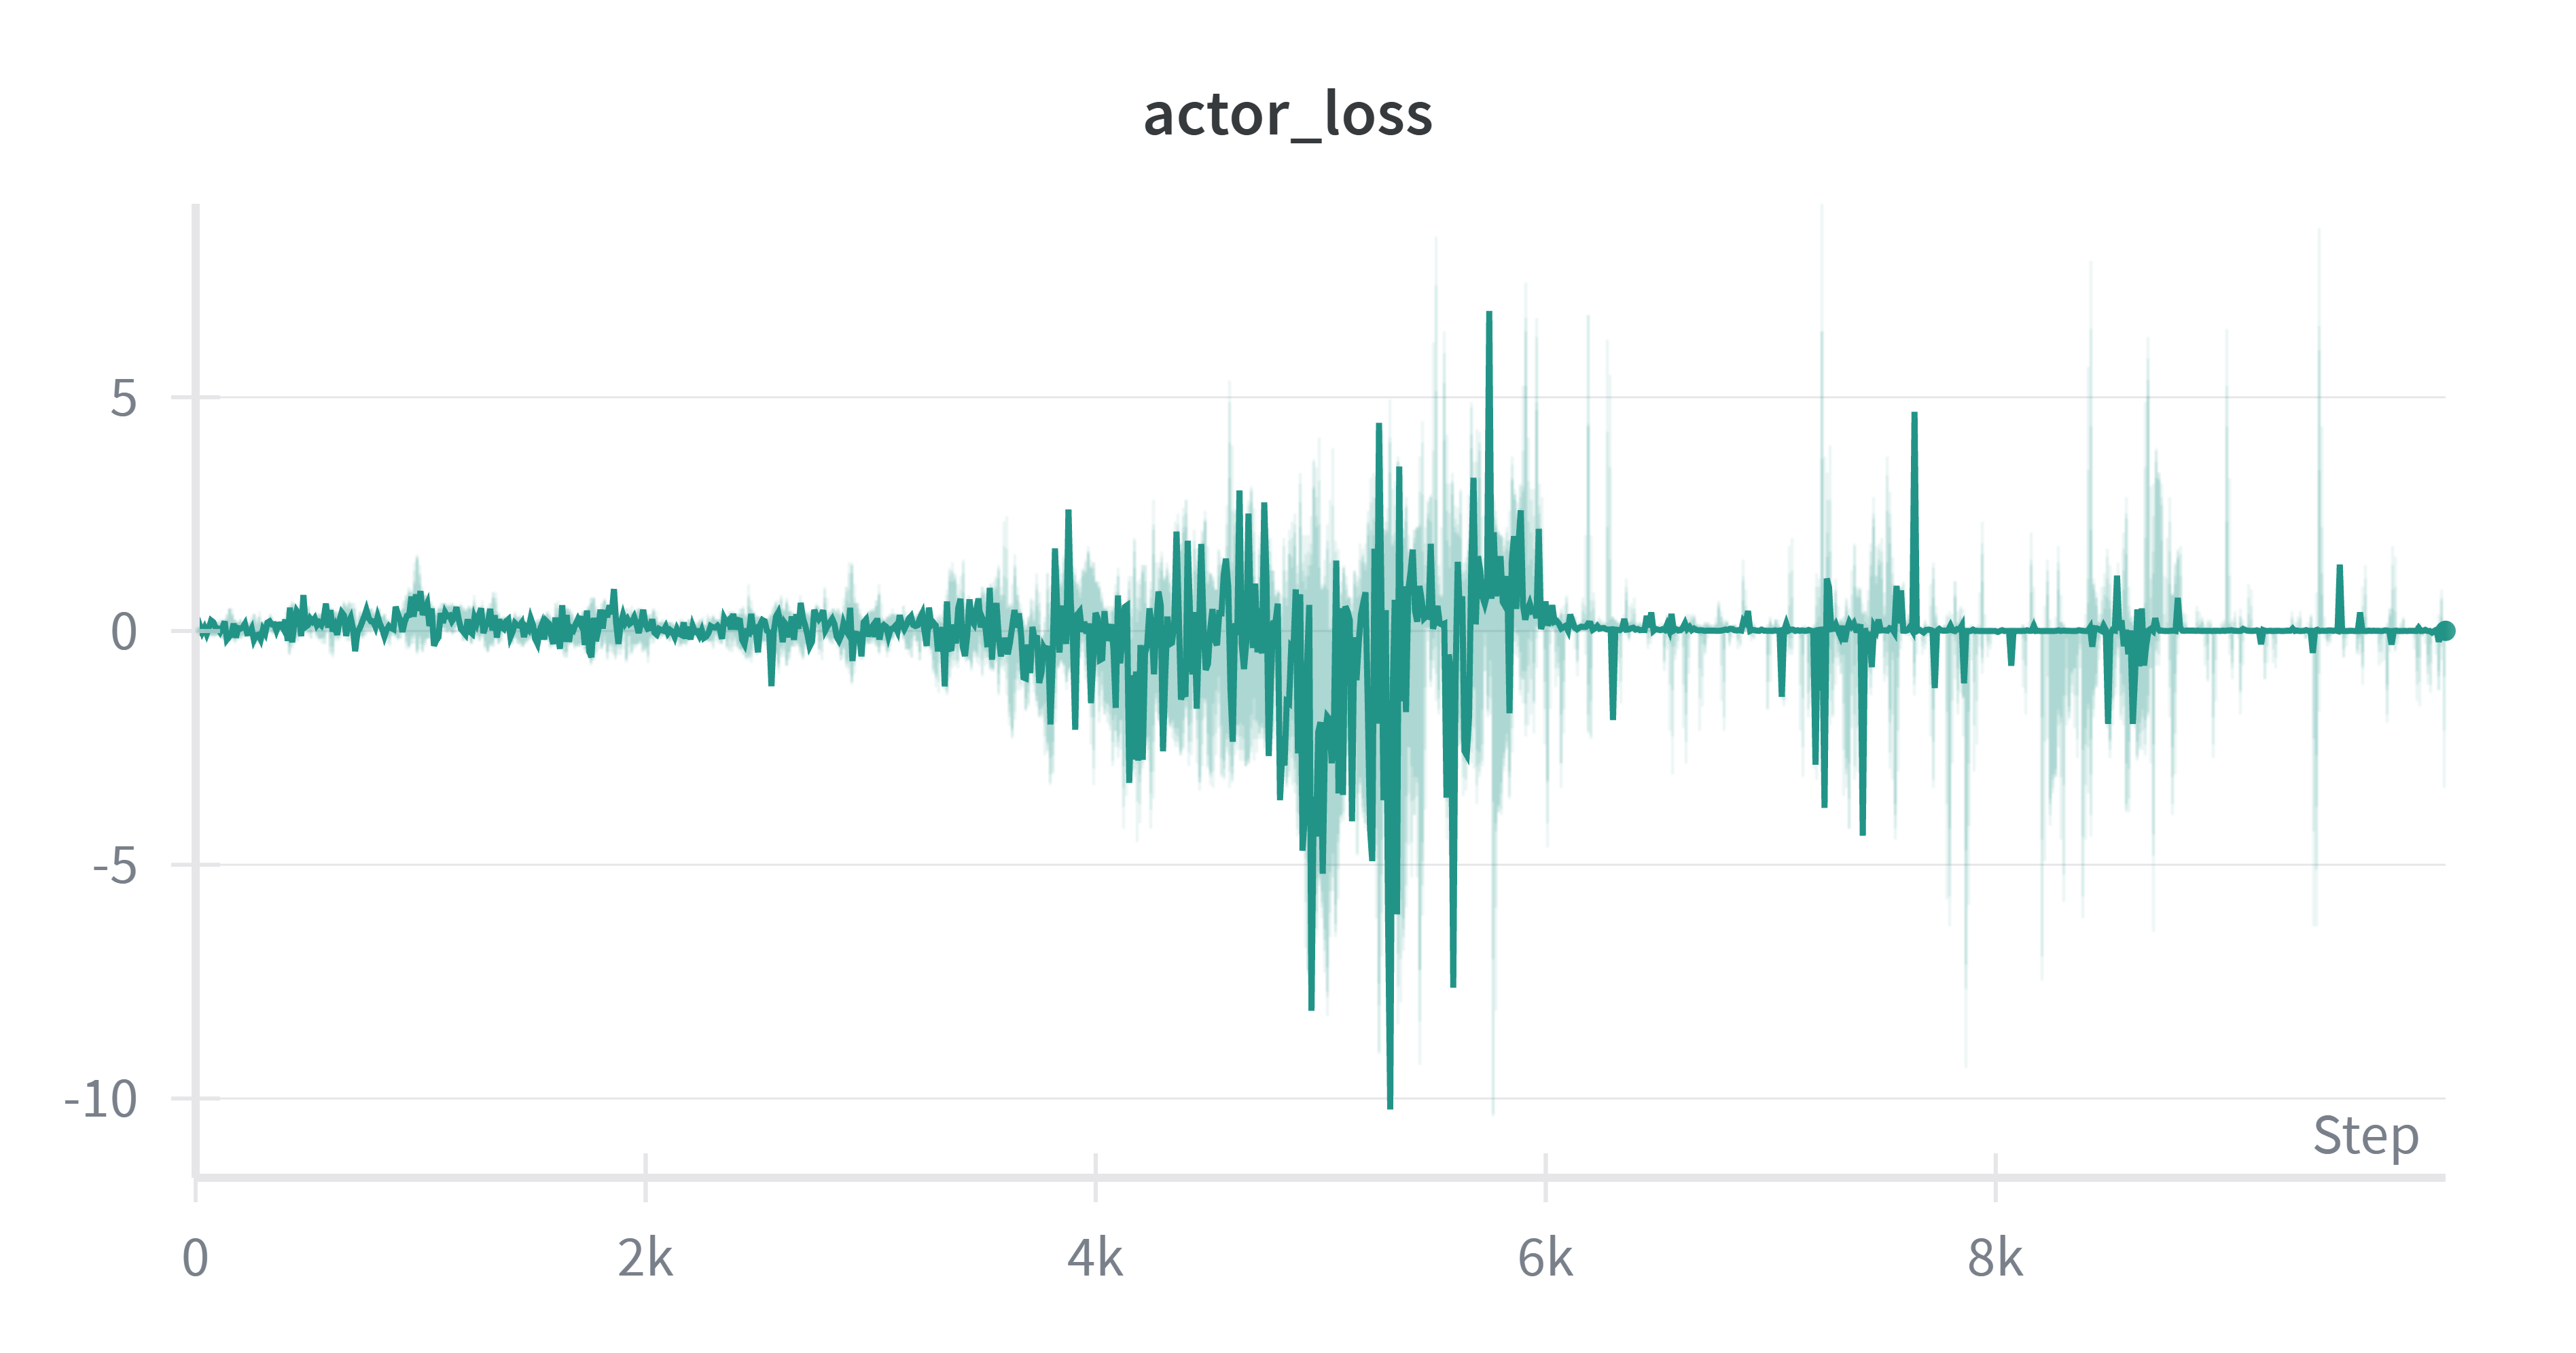
\includegraphics[width=\linewidth]{transformer_actor_loss.png}
        \caption{Transformer Actor}
    \end{subfigure}
    \caption{三种架构的 Actor Loss 变化趋势对比}
    \label{fig:actor_loss_comparison}
\end{figure}

\textbf{分析：}
\begin{itemize}
    \item \textbf{Baseline CNN}：Actor Loss 曲线非常平滑且趋近于 0，再次印证了其策略的单一性。
    \item \textbf{Transformer Actor}：Loss 曲线呈现出有节奏的震荡。结合 Transformer 最终 99\% 的胜率来看，这种震荡并非训练失败，而是策略在高维空间中不断调整优化方向的表现。相比于 CNN 的“固步自封”，Transformer 在不断尝试寻找更优的梯度方向。
\end{itemize}

\subsubsection{总结}
通过上述三组曲线的对比，我们可以得出结论：在小样本、零和博弈的强化学习任务中，\textbf{避免过早收敛}是提升最终性能的关键。虽然 Baseline CNN 训练曲线看起来平滑、收敛快，但其性能上限被锁死；而 \textbf{Transformer} 凭借其架构天然的低归纳偏置（Inductive Bias），虽然训练过程看起来高熵、高 Loss 波动，但最终学会了更复杂的全局策略，实现了性能的反超。

\end{document}